\documentclass[11pt,]{article}
\usepackage[left=1in,top=1in,right=1in,bottom=1in]{geometry}
\newcommand*{\authorfont}{\fontfamily{phv}\selectfont}
\usepackage[]{mathpazo}


  \usepackage[T1]{fontenc}
  \usepackage[utf8]{inputenc}



\usepackage{abstract}
\renewcommand{\abstractname}{}    % clear the title
\renewcommand{\absnamepos}{empty} % originally center

\renewenvironment{abstract}
 {{%
    \setlength{\leftmargin}{0mm}
    \setlength{\rightmargin}{\leftmargin}%
  }%
  \relax}
 {\endlist}

\makeatletter
\def\@maketitle{%
  \newpage
%  \null
%  \vskip 2em%
%  \begin{center}%
  \let \footnote \thanks
    {\fontsize{18}{20}\selectfont\raggedright  \setlength{\parindent}{0pt} \@title \par}%
}
%\fi
\makeatother




\setcounter{secnumdepth}{3}

\usepackage{longtable,booktabs}

\usepackage{graphicx,grffile}
\makeatletter
\def\maxwidth{\ifdim\Gin@nat@width>\linewidth\linewidth\else\Gin@nat@width\fi}
\def\maxheight{\ifdim\Gin@nat@height>\textheight\textheight\else\Gin@nat@height\fi}
\makeatother
% Scale images if necessary, so that they will not overflow the page
% margins by default, and it is still possible to overwrite the defaults
% using explicit options in \includegraphics[width, height, ...]{}
\setkeys{Gin}{width=\maxwidth,height=\maxheight,keepaspectratio}

\title{\textbar{}Estudio morfométrico fluvial de la cuenca Guayubín, República
Dominicana usando MDE de resolución y software de código abierto.  }



\author{\Large Darihana Linares Laureano\vspace{0.05in} \newline\normalsize\emph{Estudiante de Lic. en Geografía Mención Recursos Naturales y Ecoturismo,
en la Universidad Autónoma de Santo Domingo (UASD)}  }


\date{}

\usepackage{titlesec}

\titleformat*{\section}{\normalsize\bfseries}
\titleformat*{\subsection}{\normalsize\itshape}
\titleformat*{\subsubsection}{\normalsize\itshape}
\titleformat*{\paragraph}{\normalsize\itshape}
\titleformat*{\subparagraph}{\normalsize\itshape}

\titlespacing{\section}
{0pt}{36pt}{0pt}
\titlespacing{\subsection}
{0pt}{36pt}{0pt}
\titlespacing{\subsubsection}
{0pt}{36pt}{0pt}





\newtheorem{hypothesis}{Hypothesis}
\usepackage{setspace}

\makeatletter
\@ifpackageloaded{hyperref}{}{%
\ifxetex
  \PassOptionsToPackage{hyphens}{url}\usepackage[setpagesize=false, % page size defined by xetex
              unicode=false, % unicode breaks when used with xetex
              xetex]{hyperref}
\else
  \PassOptionsToPackage{hyphens}{url}\usepackage[unicode=true]{hyperref}
\fi
}

\@ifpackageloaded{color}{
    \PassOptionsToPackage{usenames,dvipsnames}{color}
}{%
    \usepackage[usenames,dvipsnames]{color}
}
\makeatother
\hypersetup{breaklinks=true,
            bookmarks=true,
            pdfauthor={Darihana Linares Laureano (Estudiante de Lic. en Geografía Mención Recursos Naturales y Ecoturismo,
en la Universidad Autónoma de Santo Domingo (UASD))},
             pdfkeywords = {Geomorfología fluvial, morfometría de cuencas, Análisis hortoniano,
Índice de concavidad, Perfil longitudinal, Patrones de drenaje},  
            pdftitle={\textbar{}Estudio morfométrico fluvial de la cuenca Guayubín, República
Dominicana usando MDE de resolución y software de código abierto.},
            colorlinks=true,
            citecolor=blue,
            urlcolor=blue,
            linkcolor=magenta,
            pdfborder={0 0 0}}
\urlstyle{same}  % don't use monospace font for urls

% set default figure placement to htbp
\makeatletter
\def\fps@figure{htbp}
\makeatother

\usepackage{pdflscape} \newcommand{\blandscape}{\begin{landscape}}
\newcommand{\elandscape}{\end{landscape}}


% add tightlist ----------
\providecommand{\tightlist}{%
\setlength{\itemsep}{0pt}\setlength{\parskip}{0pt}}

\begin{document}
	
% \pagenumbering{arabic}% resets `page` counter to 1 
%
% \maketitle

{% \usefont{T1}{pnc}{m}{n}
\setlength{\parindent}{0pt}
\thispagestyle{plain}
{\fontsize{18}{20}\selectfont\raggedright 
\maketitle  % title \par  

}

{
   \vskip 13.5pt\relax \normalsize\fontsize{11}{12} 
\textbf{\authorfont Darihana Linares Laureano} \hskip 15pt \emph{\small Estudiante de Lic. en Geografía Mención Recursos Naturales y Ecoturismo,
en la Universidad Autónoma de Santo Domingo (UASD)}   

}

}








\begin{abstract}

    \hbox{\vrule height .2pt width 39.14pc}

    \vskip 8.5pt % \small 

\noindent El estudio morfométrico de cuencas fluviales es sumamente importantes
para comprender la configuración de la misma. A pesar de esto los
estudios de esta categoría realizados en el país son muy escasos, aun
teniendo una hidrografía rica, esperando a ser explorada y analizada. El
estudio morfométrico de la cuenca Guayubín (773.56 km
extsuperscript\{2\}), señala la existencia de una relación entre la red
de drenaje con la litología el área de cuenca, que explica la forma
peculiar de la primera. De la misma manera, señala como a través de
índices es posible explicar los fenómenos descubiertos que se producen
en la cuenca, en el caso de captura fluvial. Esta investigación
evidencia la eficacia de la tecnología geoespacial para el estudio
cuantitativo de una cuenca hidrográfica, independientemente del tamaño
de la misma, así como, que esta técnica es posible aplicarla en el país
a bajo costo y produciendo información de alta calidad.


\vskip 8.5pt \noindent \emph{Keywords}: Geomorfología fluvial, morfometría de cuencas, Análisis hortoniano,
Índice de concavidad, Perfil longitudinal, Patrones de drenaje \par

    \hbox{\vrule height .2pt width 39.14pc}



\end{abstract}


\vskip 6.5pt


\noindent  \section{Introducción}\label{introducciuxf3n}

Desde hace siglos atrás el hombre ha buscado la manera de explicar y
entender las distintas formas que el paisaje terrestre (relieve) posee.
Autores numerosos han investigado la génesis de estas nociones
geomorfológicas, remontándose a tres siglos atrás. Autores como Hutton,
Playfair y Lyell, sirvieron de antecesores o bases para la ciencia
geomorfológica. Tras su consolidación como ciencia en Francia numerosos
autores fueron demostrando la importancia de esta ciencia, incluso
ramificándola (climática, eólica, litoral, glaciar, estructural,
tectónica, kárstica y fluvial; siendo la última de interés para esta
investigación), para mayor eficacia en sus estudios (Sala, 1984).

Los estudios en la geomorfología fluvial a nivel mundial son numerosos y
han servido para explicar cómo los drenajes de los ríos y sus redes
hidrográficas son importantes para la geomorfología, ya que estas redes
fluviales son parte de los procesos de modelado más activos en la
formación del relieve y que permiten mensurar la configuración del
mismo. Para los estudios en geomorfología fluvial, se hace uso del
análisis morfométrico de cuencas hidrográficas. La morfometría de cuenca
se ha convertido en la técnica cuantitativa para el estudio de las
cuencas de manera detallada y ordenada.

Actualmente en la República Dominicana el uso del análisis morfométrico
para estudiar cuencas hidrográficas es poco e insuficiente, a pesar de
que este país cuenta con una diversa y extensa red de cuencas
hidrográficas, ricas y aprovechables para la aplicación de diversas
técnicas con el fin de explicar y entender las propiedades del relieve y
su relación con las cuencas fluviales.

El aspecto general de la cuenca y de la red se refiere a los parámetros
hidrográficos que posee la cuenca y que. La forma de la cuenca y la
forma de su red de drenaje según la conformación de sus ríos y el
material rocoso que la compone (patrones de drenaje), lo que indica que
existe una conexión entre la estructura que posee la red de drenaje con
el material rocoso (Gregory \& Walling, 1973; Gutiérrez Elorza, 2008;
Howard, 1967; Pedraza Gilsanz, 1996).

El orden de red hace referencia al orden en el que se clasifican los
cursos de agua, todo en base a la magnitud de su ramificación, siendo
siempre un número entero positivo; esta clasificación se puede hacer por
mútiples normas como la de Strahler (1952), Horton (1945), Shreve
(1967), Hack (1957) y otros (Wikipedia Contributors, 2020). Para Bowden
\& Wallis (1964), el orden de red sostiene una relación entre las rocas
con la configuración de la red fluvial y con los procesos tanto
hidrológicos como erosivos. Además, la red de drenaje y el material que
transporta estan expuestos a fenómenos como la captura fluvial, que
desorienta los flujos de agua desde un lecho a otro (Pastor, 2013). Así
mismo, la razón de bifurcación (división), resulta ser la conexión entre
el número de redes fluviales de una jerarquía asignada entre el número
de redes de jerarquía mayor próxima, y señala que esta casi siempre es
constante para los órdenes de red de una cuenca (Horton, 1945).

El perfil longitudinal de un curso de agua es una línea adquirida al
representar las diversas alturas que se presentan desde el nacimiento de
este hasta donde desagua, que tiende a ser cóncavo, pero no para todos
los cursos (Gutiérrez Elorza, 2008). Por medio de los perfiles
longitudinales es posible fundamentar definiciones en segmentos con
geometría heterogénea (cóncavo, convexo y rectilíneo), o pendiente; las
acomodaciones para cada parte a una función matemática; e incluso
análisis geométricos basados en elementos físicos o evolutivos (Pedraza
Gilsanz, 1996). El índice de concavidad indica el nivel de torcedura o
curvatura del perfil longitudinal (Garzón Heydt, Ortega, Garrote, \&
others, n.d.). Se calcula así, la superficie debajo del perfil
longitudinal es extraída del total del área debajo del segmento que
conecta los dos límites del perfil (Goldrick \& Bishop, 2007).

El análisis morfométrico abarca un conjunto de índices morfológicos que
apuntan a un análisis detallado y cuantitativo de cuencas hidrográficas
(Morais \& Almeida, 2010). Donde se ordenan los canales fluviales para
establecer jerarquías y asi facilitar el estudio de la cuenca
(Christofoletti, 1988).

La curva hipsométrica de una cuenca para Strahler (1952), es un
porcentaje que explica la relación entre el área de la sección diagonal
horizontal de una red de drenaje con una altitud relativa sobre la boca
de la cuenca, e incluso estas curvas pueden ser explicadas y
relacionadas a través del uso de parámetros bidimensionales. Y referente
a la integral Hipsométrica, Fernandez \& Rocha (2016) expresa que el
cálculo de este índice mide como está distribuida la altitud en una
cuenca fluvial.

Este estudio, el primero en el campo de morfometría fluvial que se
aplica a la cuenca del río Guayubín, proporciona nueva información de la
misma sobre su configuración y modelado, y además, puede ser reproducida
sin coste alguno. Por medio de parámetros morfométricos se busca
identificar qué forma tienen la cuenca y su red de drenaje. De igual
manera, se trata de comprender como se organiza la red de drenaje y si
esta tiene algún patrón según sea su clasificación. Tras, estudiar la
cuenca y su red de drenaje, se indaga si se producen fenómenos de
reorganización en ellas, como captura fluvial o la constancia en la
razón de bifurcación. También, se inquiere sobre la existencia de una
relación entre: los perfiles longitudinales e índice de concavidad con
la litología de la cuenca; la relación entre los parámetros
morfométricos con las características litológica y estructural de
cuenca; y si hay factores que se asocien con la curva e integral
hipsométricas de la cuenca.

\section{Área de estudio}\label{uxe1rea-de-estudio}

La cuenca del río Guayubín se encuentra entre las morforegiones
Cordillera Central y Valle del Cibao Occidental, en la República
Dominicana (latitud 19.46\(^\circ\)N, longitud -71.41\(^\circ\)W), entre
las provincias Santiago Rodríguez, Monte Cristi y Dajabón. En la
provincia Dajabón engloba de forma completa el municipio El Pino, y de
manera parcial los municipios Loma de Cabrera y Partido; en la provincia
Monte Cristi contiene parcialmente los municipios Las Matas de Santa
Cruz y Guayubín; y en la provincia Santiago Rodríguez comprende los
municipios Villa Los Almácigos y San Ignacio de Sabaneta. Los municipios
más poblados en el interior de la cuenca son Guayubín (35,923 hab.), San
Ignacio de Sabaneta (34,540 hab), y Loma de Cabrera (15,624 hab). (Ver
figura \ref {mapacuenca}).

La cuenca del río Guayubín, según Medio Ambiente y Recurso Naturales
(2015), abarca una área de 770.35 km\textsuperscript{2}. De acuerdo con
el mapa de Medio Ambiente y Recurso Naturales (2015), la cabecera del
rio Guayubín se ubica en la vertiente noroeste del Cerro La Pelada, en
un paraje denominado Palo Amarillo; mientras que sus aguas se vierten en
el río Yaque del Norte, en la localidad Guayubín.

\section{Materiales y Metodología}\label{materiales-y-metodologuxeda}

Para este estudio se utilizaron operaciones de análisis morfométrico de
redes de drenaje y cuenca de los paquetes de software de código abierto
Grass Gis (Neteler, Beaudette, Cavallini, Lami, \& Cepicky, 2008) por
medio de entorno de programación R (Allaire, 2012). Todos los análisis
de carácter estádisticos y las figuras de los resultados, fueron
realizadas en R usando diversos paquetes (ver tabla
\ref{tab:materiales}). Se utilizó un modelo digital de elevaciones (en
lo adelante, \texttt{MDE}), de la misión tadar del transbordador
espacial Shttle (Farr et al., 2007), a 90 metros de resolución, para
extraer los datos a analizar e interpretar.

Los parámetros de la cuenca fueron calculados por medio del addon de
GRASS GIS \texttt{r.watershed} (Ehlschlaeger \& Laboratory,
2003--2021b), utilizando un Dem. Las capas generadas fueron ingresadas a
R con la librería \texttt{sp} y manejadas con la librería
\texttt{raster}.

Se usó el addon \texttt{r.water.outlet} (Ehlschlaeger \& Laboratory,
2003--2021a) para la extracción de la cuenca. Así mismo, se usó el addon
\texttt{r.to.vect} (GRASS Development Team, 2003--2021), para convertir
el ráster resultante en vectorial; todos los resultados, generados por
estos dos addons, fueron llevados a R.

Para extraer la red de drenaje se aplicó el addon
\texttt{r.stream.extract} (Metz, 2003--2021), y luego, fueron llevados a
R.

En cuanto al orden de red y el análisis hortoniano, se usó el addon
\texttt{r.stream.extract} (Metz, 2003--2021), para producir un mapa de
dirección de flujo. Para la creación de mapas de ordenes de redes se
utilizó el addon \texttt{r.stream.order} (J. Jasiewicz, 2003--2021).

Para analizar el orden de red de la cuenca se utilizó la clasificación
de Strahler, generada con (J. Jasiewicz, 2003--2021). Mientras que, se
usaron los addons \texttt{r.info} (O'Shea \& Laboratory, 2003--2021),
para obtener los valores mínimos y máximos del orden de red según
Strahler a partir de un ráster.

Para delimitar la cuenca a través de la red de drenaje se utilizó
\texttt{r.stream.basins} (J. Jasiewicz, University, Geoecology, \&
Institute, 2003--2021). En cuanto a las estadísticas según orden de red
de Horton para las redes de Strahler y Horton, se usó el addon
\texttt{r.stream.stats} (j. Jasiewicz, University, \& Geoinformation
Institute, 2003--2021), para resumir las estadísticas.

Para calcular los índices de concavidad y los perfiles longitudinales,
primero, se obtuvieron los cursos más largos de la cuenca a través de la
función \texttt{LfpNetwork} (José Ramón Martínez Batlle, 2018b). Y
segundo, para producir los perfiles longitudinales e índices de
concavidad se empleó la función \texttt{LfpProfilesConcavity} (José
Ramón Martínez Batlle, 2018c).

Tras crear una nueva región de GRASS en R, se convirtieron a números
enteros la extensión y la resolución del DEM con las funciones
\texttt{integerextent} (José Ramón Martínez Batlle, 2020a), y
\texttt{xyvector} (José Ramón Martínez Batlle, 2018d). También, se usó
la herramienta \texttt{gdalwarp} (Warmerdam, Rouault, \& others,
1998--2021), para reproyectar y deformar ráster. Se utilizaron los
addons \texttt{g.proj} (Kelly, 2003--2021), y \texttt{r.in.gdal}
(Warmerdam, 2003--2021), para importar a la sesión de GRASS. Se usó el
addon \texttt{r.stream.extract} (Metz, 2003--2021), para generar una red
de drenaje y obtener coordenadas a continuación, y que serían, luego,
transformadas a EPSG: 4326 (Lohmar, 1988), como número entero con la
función \texttt{My\_Trans} (José Ramón Martínez Batlle, 2020b).

En cuanto a la obtención de los parámetros morfométricos de la cuenca se
usa el addon \texttt{r.basin} (Di Leo \& Di Stefano, 2003--2021). Los
vectores obtenidos son transformados a EPGS: 4326 (Lohmar, 1988), y asi
visualizados con la librería \texttt{leaflet}. También, para explorar
los parámetros de la cuenca se usó la librería \texttt{readr}.

Finalmente, para el cálculo de la curva y la integral hipsométrica, lo
primero fue representar las cuencas con las librerías \texttt{sp} y
\texttt{mapview}; y segundo, calcular la integral y curva hipsométrica
utilizando la función \texttt{HypsoIntCurve} (José Ramón Martínez
Batlle, 2018a).

\section{Resultados}\label{resultados}

El fruto del estudio realizado a la cuenca del río Guayubín aplicando la
metodología anterior, produce información que facilita el análisis y
comprensión de la cuenca fluvial, tanto de manera agrupada, como de
forma desagregada.

\subsection{Aspecto general de la cuenca y de la red de
drenaje.}\label{aspecto-general-de-la-cuenca-y-de-la-red-de-drenaje.}

Los resultados arrojados por el estudio muestran que la cuenca del río
Guayubín tiene una área de 773.56 km\textsuperscript{2}, y un perímetro
de 156.12 km (Ver tablas \ref{tab:estadisticaor} y
\ref{tab:parametrosm}). La cuenca tiene forma de pera y su red drenaje
presenta patrones dendríticos (ver figura
\ref{red de drenaje extraida}).

\subsection{Orden de red analisis
hortoniano}\label{orden-de-red-analisis-hortoniano}

El orden de red de cada tramo fluvial de la cuenca según Strahler,
indicó que el orden de red máximo (5) y el mínimo (1). (ver figura
\ref{unica}, y figura \ref{subcuencas}). Las estadísticas por orden de
red según la clasificación de Strahler, obtenidas con
\texttt{r.stream.stats} indican que el número total de redes en la
cuenca es de 367, tambien se obtuvieron el total longitud por órdenes de
red resultando en 693.61 km (ver tabla \ref{tab:estadisticaor}). De la
misma manera se generó el dato de la razón de bifurcación para la red
basada en el coeficiente de regresión es de 4.1, también se obtuvieron
resultados de razón de bifurcación para cada orden de red, para el redes
de orden 1 (4.7), de orden 2 (3.6), orden 3 (4.3), para los de orden 4
(4), y para los de orden 5 (0), las otras estadísticas están detalladas
en la tabla \ref{tab:estadisticaor} y sus derivadas en esta figura (ver
figura \ref{grafnumero}). Como se observa en las tablas
\ref{tab:regresionc} y ref \{tab:estandard\}, las razones de bifurcación
se obtuvieron razones de bifurcación con criterios distintos. Otras
estadísticas como la longitud promedio y area promedio para cada orden
de red estas detalladas en la tabla \ref{promo}. También, se obtuvieron
las estadísticas de la desviación estándar de ares y longitudes por
orden de red, ver tabla \ref{estad}. De igual manera se generaron las
estadísticas de los parámetros hidrográficos (número de orden, longitud
y áreas), según el orden de red (ver tabla \ref{parh}). En tabla
\ref{razones}, se presentan los valores resultantes para la razón de
bifurcación.

\subsection{Índices de concavidad y perfiles
longitudinales}\label{uxedndices-de-concavidad-y-perfiles-longitudinales}

Con la función \texttt{LfpNetwork} se obtuvieron los cursos más largos
de la red de drenaje, siendo un total de 60 cursos. De los cuales los
cursos 30, 48, 52, 55 y 56 (0.59; 0.51; 0.51; 0.54; y 0.47,
respectivamente), presentaron los más altos índices de concavidad;
siendo el curso 30 el poseedor del índice de concavidad más alto de
todos los cursos. Mientras que los cursos de agua 15, 16, 23 y 38
presentaron valores menores a 0.03, poseyendo los valores as bajos de
todos los cursos (ver figura \ref{lfpnet}, \ref{plongitudinal} y
\ref{indicec}).

\subsection{Morfometría de cuenca}\label{morfometruxeda-de-cuenca}

Los parámetros morfométricos obtenidos con \texttt{r.basin}, indicaron
que la elevación mínima en la cuenca del rio Guayubín fue 30.97 mslm y
la maxima fue 1396.73 mslm, mientras la diferencia de elevación obtenida
de los cálculos fue de 1365.76 m. Asi mismo, se produjo el parámetro de
elevación media (276.70). El parámetro de coeficiente de compacidad
obtenido fue de 4.9. El curso mas largo de la red de drenaje o curso
principal en la cuenca producido por \texttt{r.basin} presento una
longitud de 61.96 km. El resto de los parámetros obtenidos están
resumidos en la tabla \ref{tab:parametrosm}.

Las estadísticas que se generaron sobre la curva y la integral
hipsométrica se obtuvieron 60 resultados para los cursos de agua
pertenecientes a la cuenca de orden 2. El valor mínimo generado para la
integral hipsométrica fue 0.08 en el curso 43. En tanto, el valor máximo
para la integra fue de 0.48 en el curso 45 (ver tabla \ref{ihco2}). los
cursos más curvos fuero 37, 18 y 15. Ver figuras\ref{hypsob2} y
\ref{hypb2}.

En cuanto a las cursos de agua de las cuencas de orden 3, se produjeron
17 resultados, donde los cursos 8 (0.40), 11 (0.34), y 13 (0.33),
presentaron los valores de integral hipsométrica más altos. Y los cursos
con los valores más bajos de la integral hipsométrica fueron 4 (0.12), y
16 (0.06). Ver tabla \ref{ihco3}. y los cursos más curvos obtenidos
fueron 5, 10, 17, y 18. Ver figuras \ref{hysob3} y \ref{hypb3}.

\section{Discusión}\label{discusiuxf3n}

Con los hallazgos producidos sobre la cuenca del rio Guayubín, es
posible responder a las preguntas planteadas sobre la forma de la cuenca
y su red de drenaje, los patrones en la red de drenaje, la organización
de la red de drenaje, el fenómeno de constancia, la relación de los
perfiles longitudinales y su índice de concavidad con la litología en la
cuenca, la relación de los parámetros de cuenca con la litología, al
igual que la relación de la curva hipsométrica y la integral con la
litología. Además, es posible hacer comparaciones de eficacia del método
empleado para extraer las redes de drenaje con el mapa topológico de
República Dominicana (Lizmap, s.f.).

En los parámetros de cuenca y en las estadísticas de ordenes de red, el
valor de área de cuenca se mantuvo sin cambios; pero comparándolos con
las informaciones extraídas de Medio Ambiente y Recurso Naturales (2015)
los valores que se obtuvieron no concuerdan, puesto que, la cuenca
presentada por Medio Ambiente y Recurso Naturales (2015) es más pequeña
que la producida por los algoritmos en R (ver tablas
\ref{tab:parametrosm} y \ref{tab:estadisticaor}.

La cuenca tiene forma de pera (Terrain Works Team, 2014) y la forma de
su red de drenaje es dendrítica (Gutiérrez Elorza, 2008). La forma de la
red de drenaje se produce en zonas de relieve heterogéneo como se
presenta la parte de cuenca alta; los cursos de agua se desarrollan
libremente y no depende de un control estructurales (Ingeniero Civil
Team, 2018); la cuenca esta acentuada en rocas de tipo ígneas o
magmáticas y sedimentarias (Mollat, Wagner, Cepek, \& Weiss, 2004).
Howard (1967) asegura que los patrones dendríticos los sedimentos tienen
una resistencia uniforme.

La red de drenaje de la cuenca presenta signos de haber sufrido el
fenómeno de reorganización captura fluvial, según Pastor (2013) este
fenómeno se puede identificar al observar la red de drenaje, donde se
producen cambios abruptos en el recorrido del cauce que ha sido captura.
Se ha observado que este fenómeno se produce en todas las redes desde
orden 1 a orden 5, en especial en las redes de orden más bajo, pero
puede verse muy marcado en la red de orden cinco, donde se produce
cambios del tipo de roca y relieve es má heterogéneo (ver figura
\ref{grosor} y \ref{magecu}).

Según Summerfield (1991), la razón de bifurcación que esta entre 3 y 5,
indica que la litología del lugar es homogénea. En tabla \ref{razones},
es visible como los valores para la razón de bifurcación en los órdenes
de red difieren el uno del otro, los órdenes 1, 2, 3 y 4 mantienen una
homogeneidad en su litología. Como se observa en las tablas
\ref{tab:regresionc} y ref\{tab:estandard\}, las razones de bifurcación
obtenidas se corresponden. Ambos valores coinciden con la razón de
bifurcación calculada con código en R (4.064346), podemos concluir que
mantienen una constancia en el tipo de roca presente.

Los cursos más largos de la red de drenaje que tienen los más altos
índices de concavidad fueron los cursos 30, 48, 52, 55 y 56 (0.59; 0.51;
0.51; 0.54; y 0.47, respectivamente), lo que indica que hubo un cambio
en el trayecto que recorren esos cursos de agua que esté relacionado a
la aparición de una roca dura, tras haber comparado los resultados de
los cursos más largo en el mapa geológico nacional (Mollat et al.,
2004), se comprueba que existe un cambio en la litología presente en los
cursos de agua, en el caso del curso 30 con un índice de 0.59 de
concavidad, al pasar de estar sobre rocas tonalitas a estar sobre rocas
sedimentarias y de originadas en arcos de islas se produce un cambio en
su trayectoria. También se vio afectado el curso de agua 19, quien
presenta un índice de concavidad de 0.46 producto de que este flujo en
su trayecto se encuentra con una falla tectónica, provocando el cambio
en su curso. Y los cursos más rectilíneos con los índices de concavidad
más bajos son los cursos de agua número 15, 16, 23 y 38, con valores
menores a 0.03, estos cursos de agua realizan su recorrido por un mismo
tipo de roca por lo que no experimenta cambios bruscos en su curso (ver
figura \ref{lfpnet}, \ref{plongitudinal} y \ref{indicec}).

Los parámetros morfométricos obtenidos con \texttt{r.basin} (ver tabla
\ref{parametrosm}), indican que la elevación mínima en la cuenca del rio
Guayubín es 30.97 mslm y la máxima es 1396.73 mslm, por lo que existe
una diferencia de elevación en la cuenca de 1365.76 m; mientras que su
elevación media fue de 276.70. El parámetro coeficiente de compacidad es
4.9 lo que indica que la forma de la superficie de la cuenca de acuerdo
con su delimitación, y el predominio en su escorrentía, es muy alargada
(López Cadenas de Llano \& Mintegui Aguirre (1986)); pero, el parámetro
forma de la cuenca genero un índice de 12.48 lo que indica que la cuenca
además de ser muy alargada está bastante ensanchada en las zonas de
cuenca alta y cuenca media (Córdova, 2016; Pérez, 1979). Según los
resultados de la razón de elongación (0.50), se confirma que la cuenca
es alargada (De Matauco, 2004).

El curso más largo de la red de drenaje o curso principal en la cuenca,
producido por \texttt{r.basin} tiene una longitud 61.96 km; según una
comparación realizada entre el vectorial de cursos más largo (ver figura
\ref{lfpnet}), y el curso que se obtuvo con \texttt{r.basin} (ver figura
\ref{vectoresrbasin}), es el curso numero 30 obtenido con la función
\texttt{LfpNetwork}. Por lo que la cabecera del rio Guayubín se localiza
al sureste de la indicada por Medio Ambiente y Recurso Naturales (2015),
bajo el nombre de Dajao.

La curva y la integral hipsométrica muestran la repartición de
elevaciones en la cuenca (Jose Ramon Martinez Batlle, 2019). El valor
mínimo generado para la integral hipsométrica fue 0.08 en el curso 43.
En tanto, el valor máximo para la integra fue de 0.48 en el curso 45
(ver tabla \ref{ihco2}). Y los cursos más curvos fueron 37 y 18. El
primero presenta signos de una evolución lenta en su elevación; y el
segundo, presenta una evolución media en su elevación. Ver figuras
\ref{hypsob2} y \ref{hypb2}. Los cursos 41 y 42 son los más rectilíneo y
su integral hipsométrica es moderada por lo que estos cursos han
experimentado poca evolución rápida en su elevación.

Los cursos de agua pertenecientes a la cuenca de orden 3, los valores
máximos presentes (8 y 13), tuvieron una evolución media en la
elevación. Y los cursos 4 y 16, demuestran una lenta y estable evolución
en la elevación (ver tabla \ref{ihco3}). Ver figuras \ref{hysob3} y
\ref{hypb3}.

Toda la información generada sobre la cuenca sirve como peldaño a
futuras investigaciones sobre la misma u otras cuencas fluviales en el
país.

El estudio está limitado a los análisis cuantitativos, puesto que carece
de la toma de muestras en campo para una más precisa comprensión de la
cuenca.

\section{Agradecimientos}\label{agradecimientos}

A Dios por la fuerza y la salud que me ha dado durante todo este tiempo,
sin dejarme caer.

A mi maestro \texttt{Jose\ Martínez\ Batlle} por el apoyo incondicional,
tanto emocional como técnico, por ser guía durante todo el trayecto, por
ser paciente, y sobre todo por su disponibilidad para colaborar.

A mi compañero de carrera y amigo \texttt{Welifer\ Lebron} por su
asesoramiento.

A mis compañeros
\texttt{Saderis\ Carmona,\ Franklin\ Gomez,\ Randy\ Mueses,\ Frank\ de\ la\ Cruz\ y\ Cinthia\ Vandepool}
quienes estuvieron presente en este nuevo reto en el que nos embarcamos
tres meses atrás, y de los cuales he recibido apoyo emocional y técnico,
también por sus maneras de ayudarnos entre si a liberar estrés.

A mi madre \texttt{Denny\ Laureano}, mis hermanos
\texttt{Darleny\ Linares,\ Diana\ Carolina\ Linares\ y\ Jose\ Daniel\ Linares}
por la comprensión y el apoyo tanto moral como emocional durante este
tiempo.

A mis amistades por el apoyo, comprensión y motivación para que continúe
mis proyectos.

\section{Información de soporte}\label{informaciuxf3n-de-soporte}

\begin{figure}
\centering
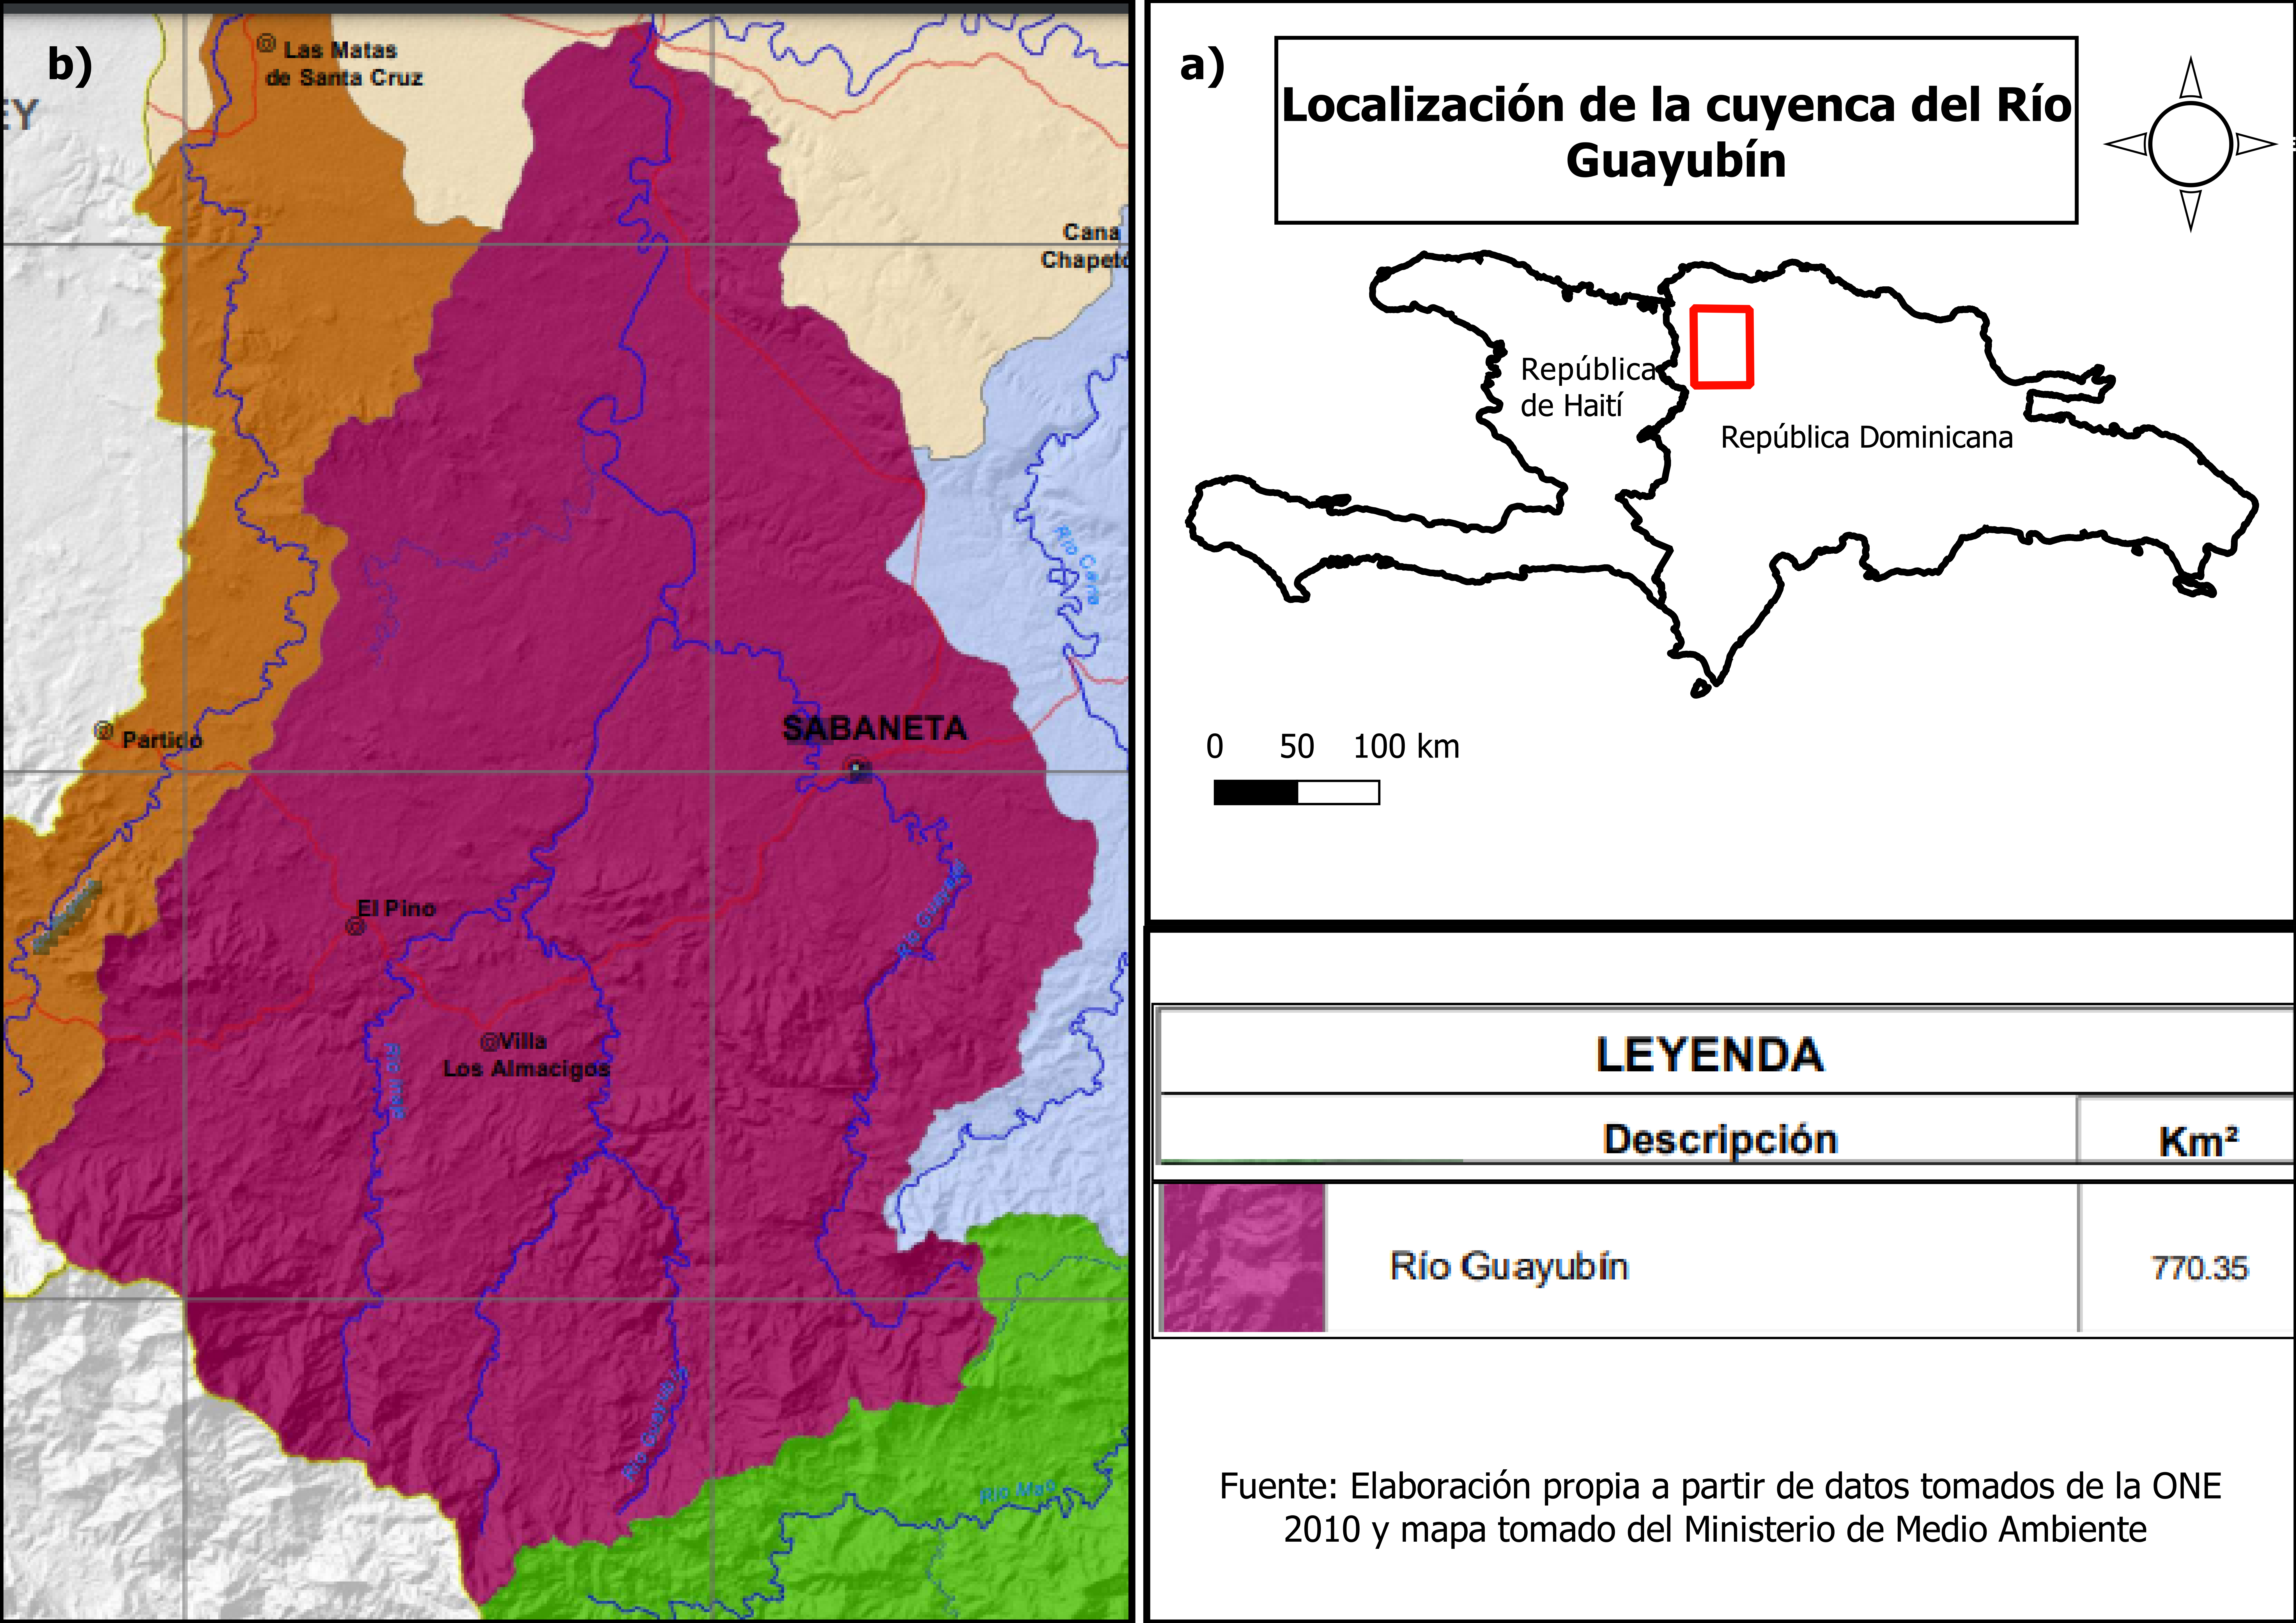
\includegraphics[width=1.00000\textwidth]{Mapa final.png}
\caption{Cuenca del río Guayubín\label{mapacuenca}}
\end{figure}

\begin{figure}
\centering
\includegraphics[width=0.60000\textwidth]{geologico.png}
\caption{Mapa Geologico de la cuenca\label{magecu}}
\end{figure}

\begin{figure}
\centering
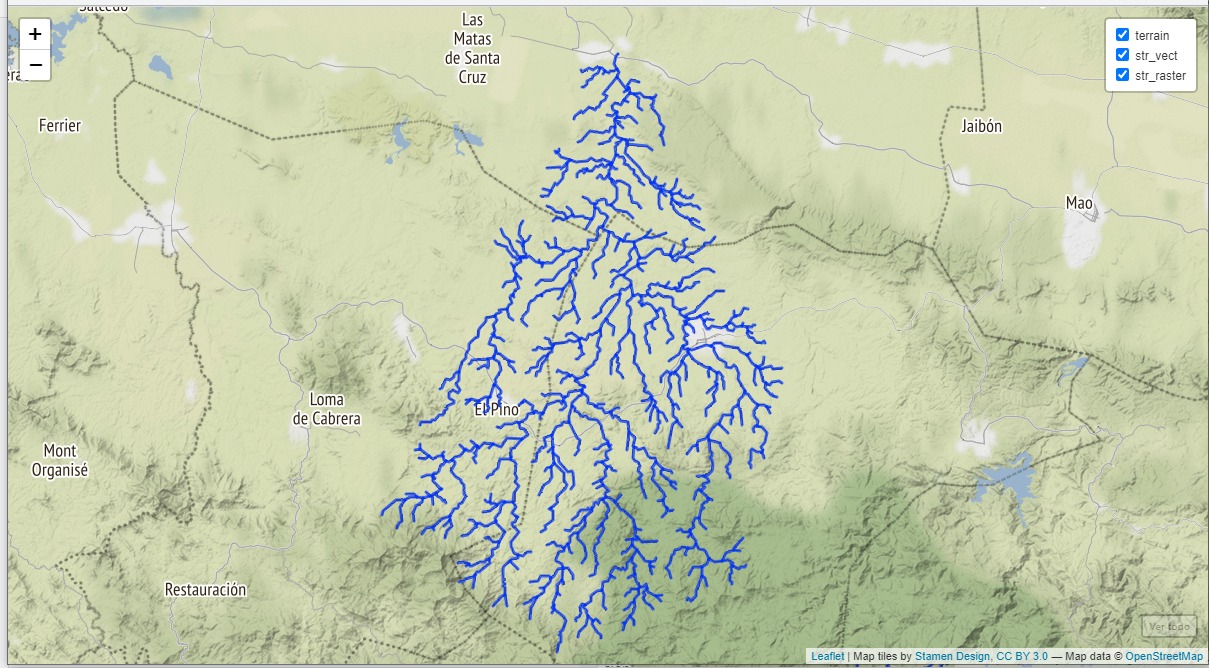
\includegraphics[width=0.70000\textwidth]{red de drenaje extraida.png}
\caption{Red de drenaje del río Guayubín\label{red de drenaje extraida}}
\end{figure}

\begin{figure}
\centering
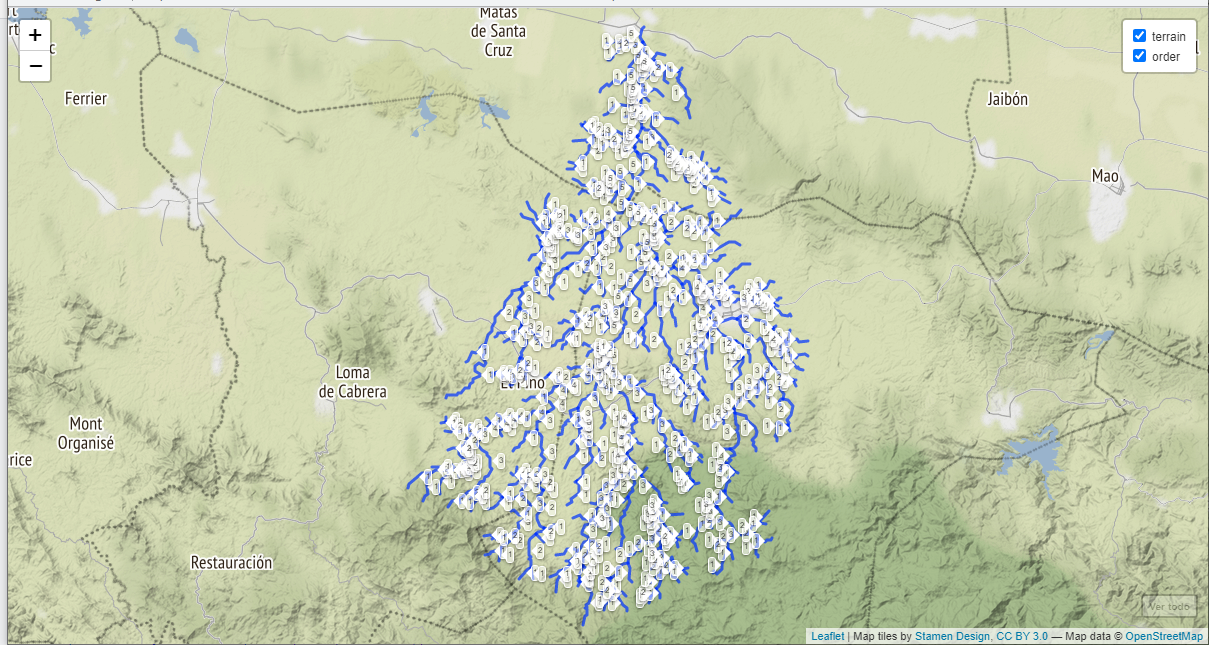
\includegraphics[width=1.00000\textwidth]{ordenes de red.png}
\caption{Ordenes de red del río Guayubín con simbología
única\label{unica}}
\end{figure}

\begin{figure}
\centering
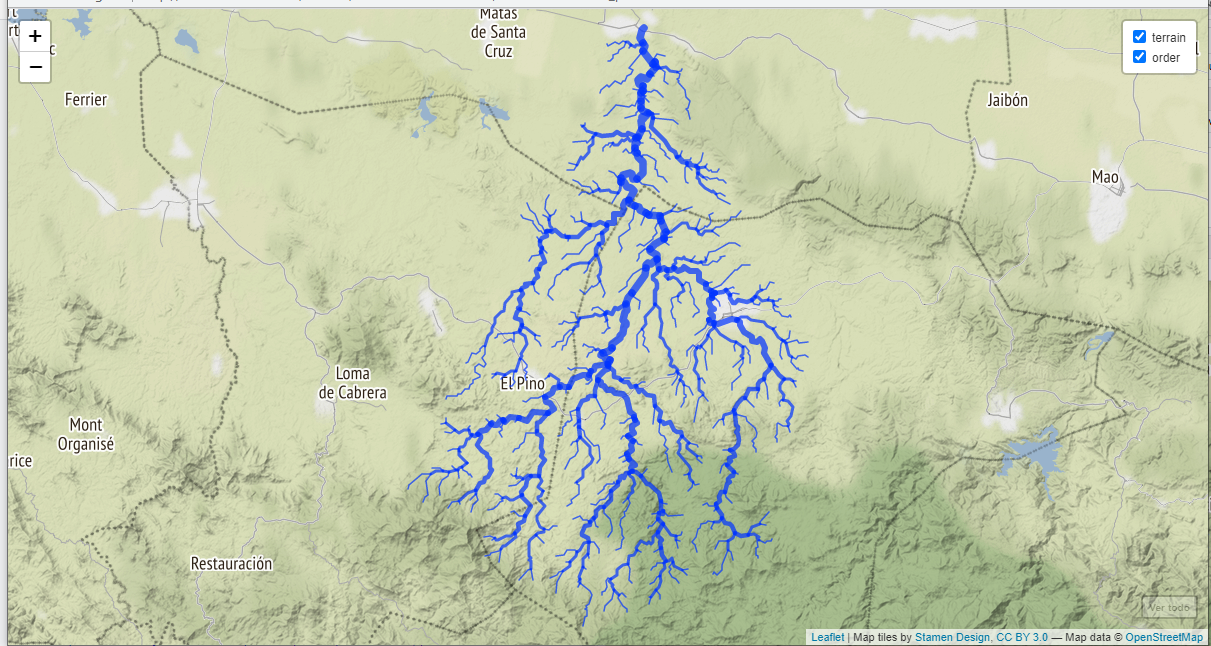
\includegraphics[width=0.80000\textwidth]{orden de red mapa 2.png}
\caption{Ordenes de red del río Guayubín con simbología aplicando grosor
según su orden\label{grosor}}
\end{figure}

\begin{figure}
\centering
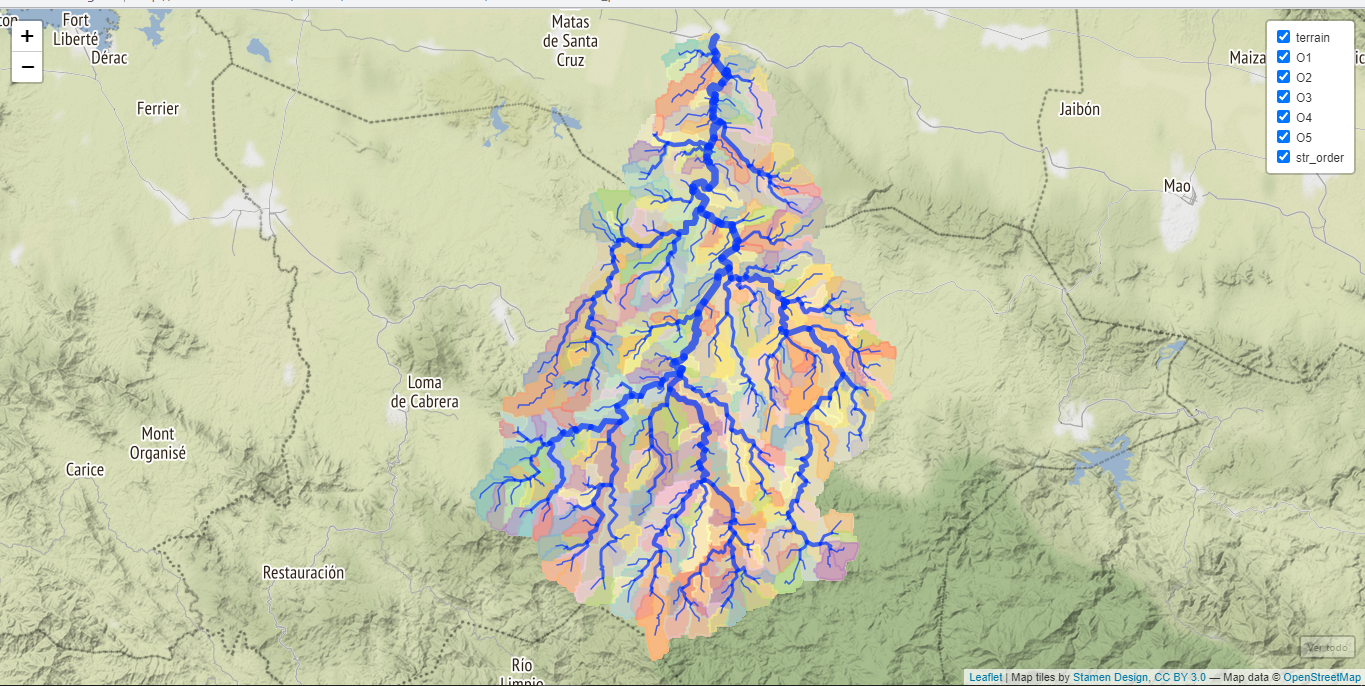
\includegraphics[width=0.70000\textwidth]{cuencas delimitadas y ordenes de red.png}
\caption{Subcuencas y ordenes de red del río Guayubín\label{subcuencas}}
\end{figure}

\begin{figure}
\centering
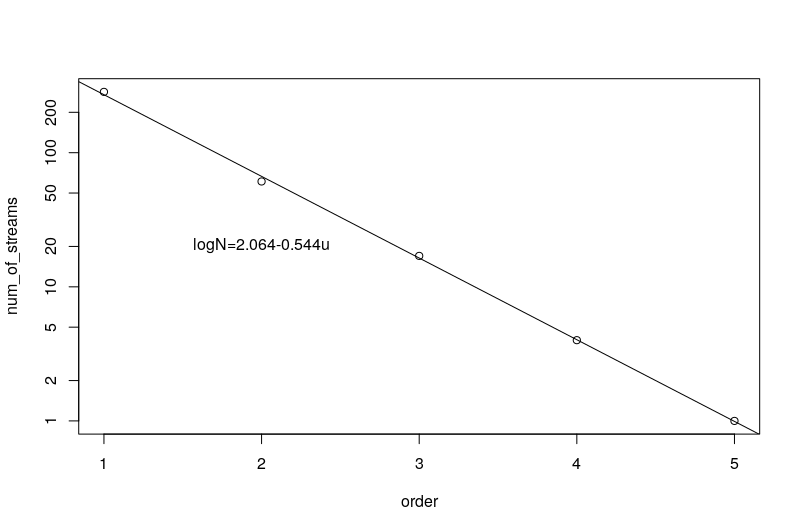
\includegraphics[width=0.80000\textwidth]{Numero de red segun su orden.png}
\caption{Número de redes según su orden y Razón de
bifurcación\label{grafnumero}}
\end{figure}

\begin{figure}
\centering
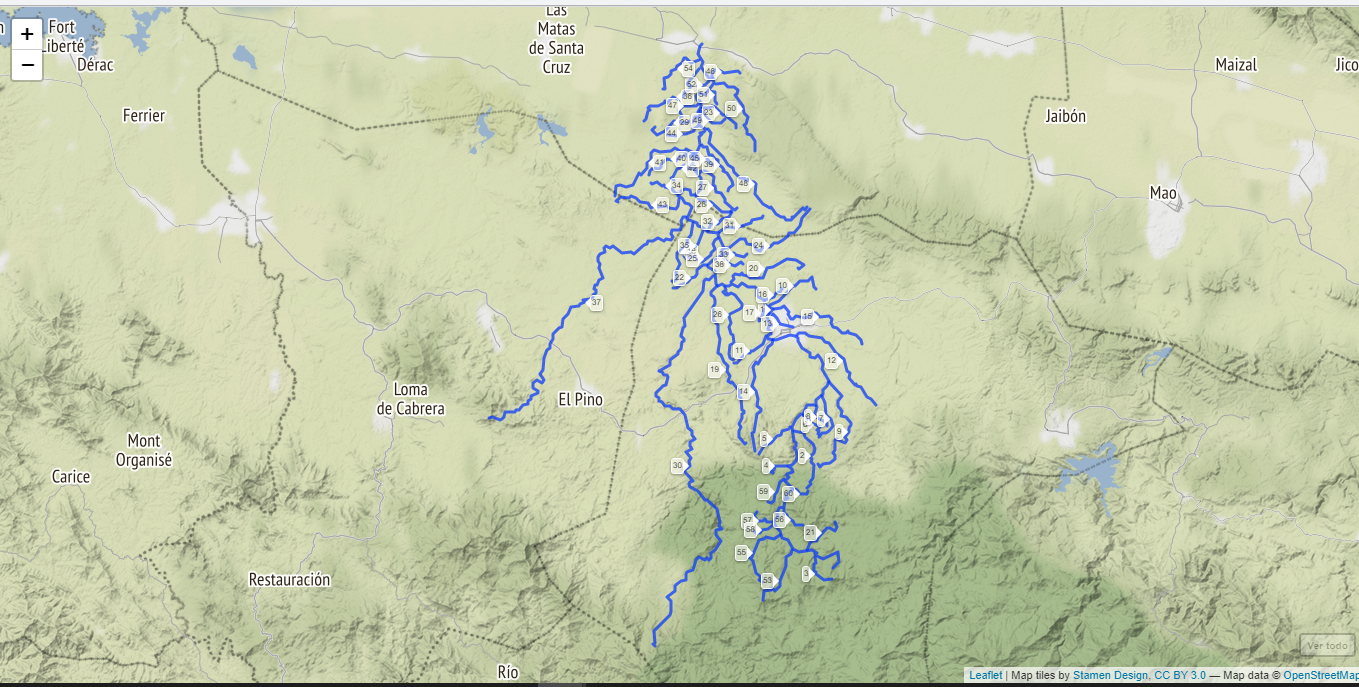
\includegraphics[width=1.00000\textwidth]{cursos mas largos.png}
\caption{Cursos fluviales mas largos de la cuenca del río
Guayubín\label{lfpnet}}
\end{figure}

\begin{figure}
\centering
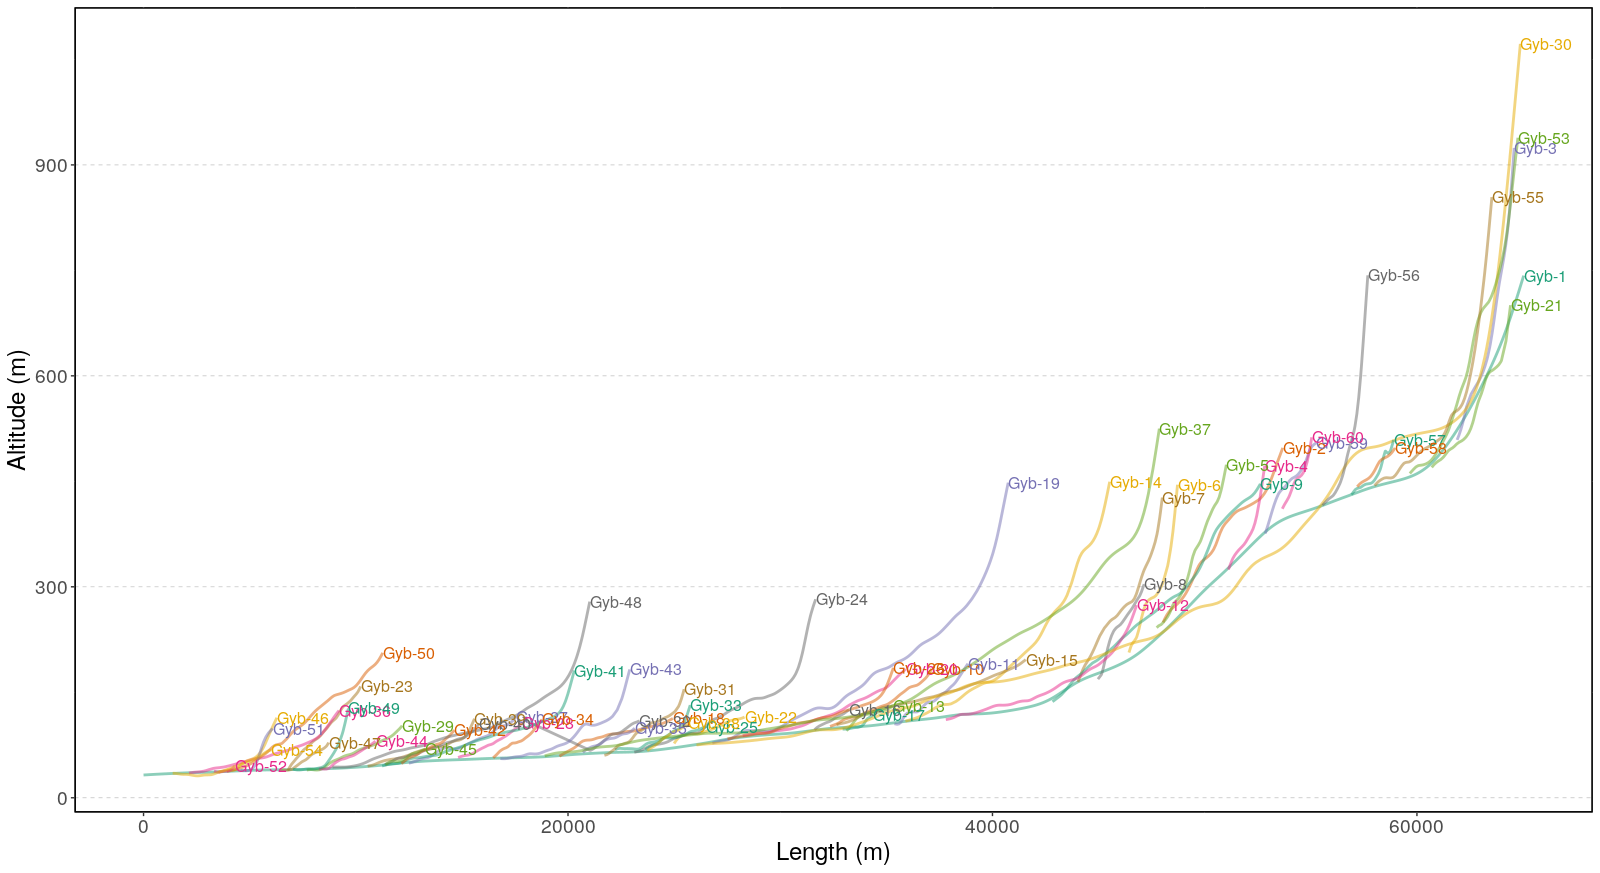
\includegraphics[width=1.00000\textwidth]{perfiles longitudinales.png}
\caption{Perfiles longitudinales de los cursos más largos en la cuenca
del río Guayubín\label{plongitudinal}}
\end{figure}

\begin{figure}
\centering
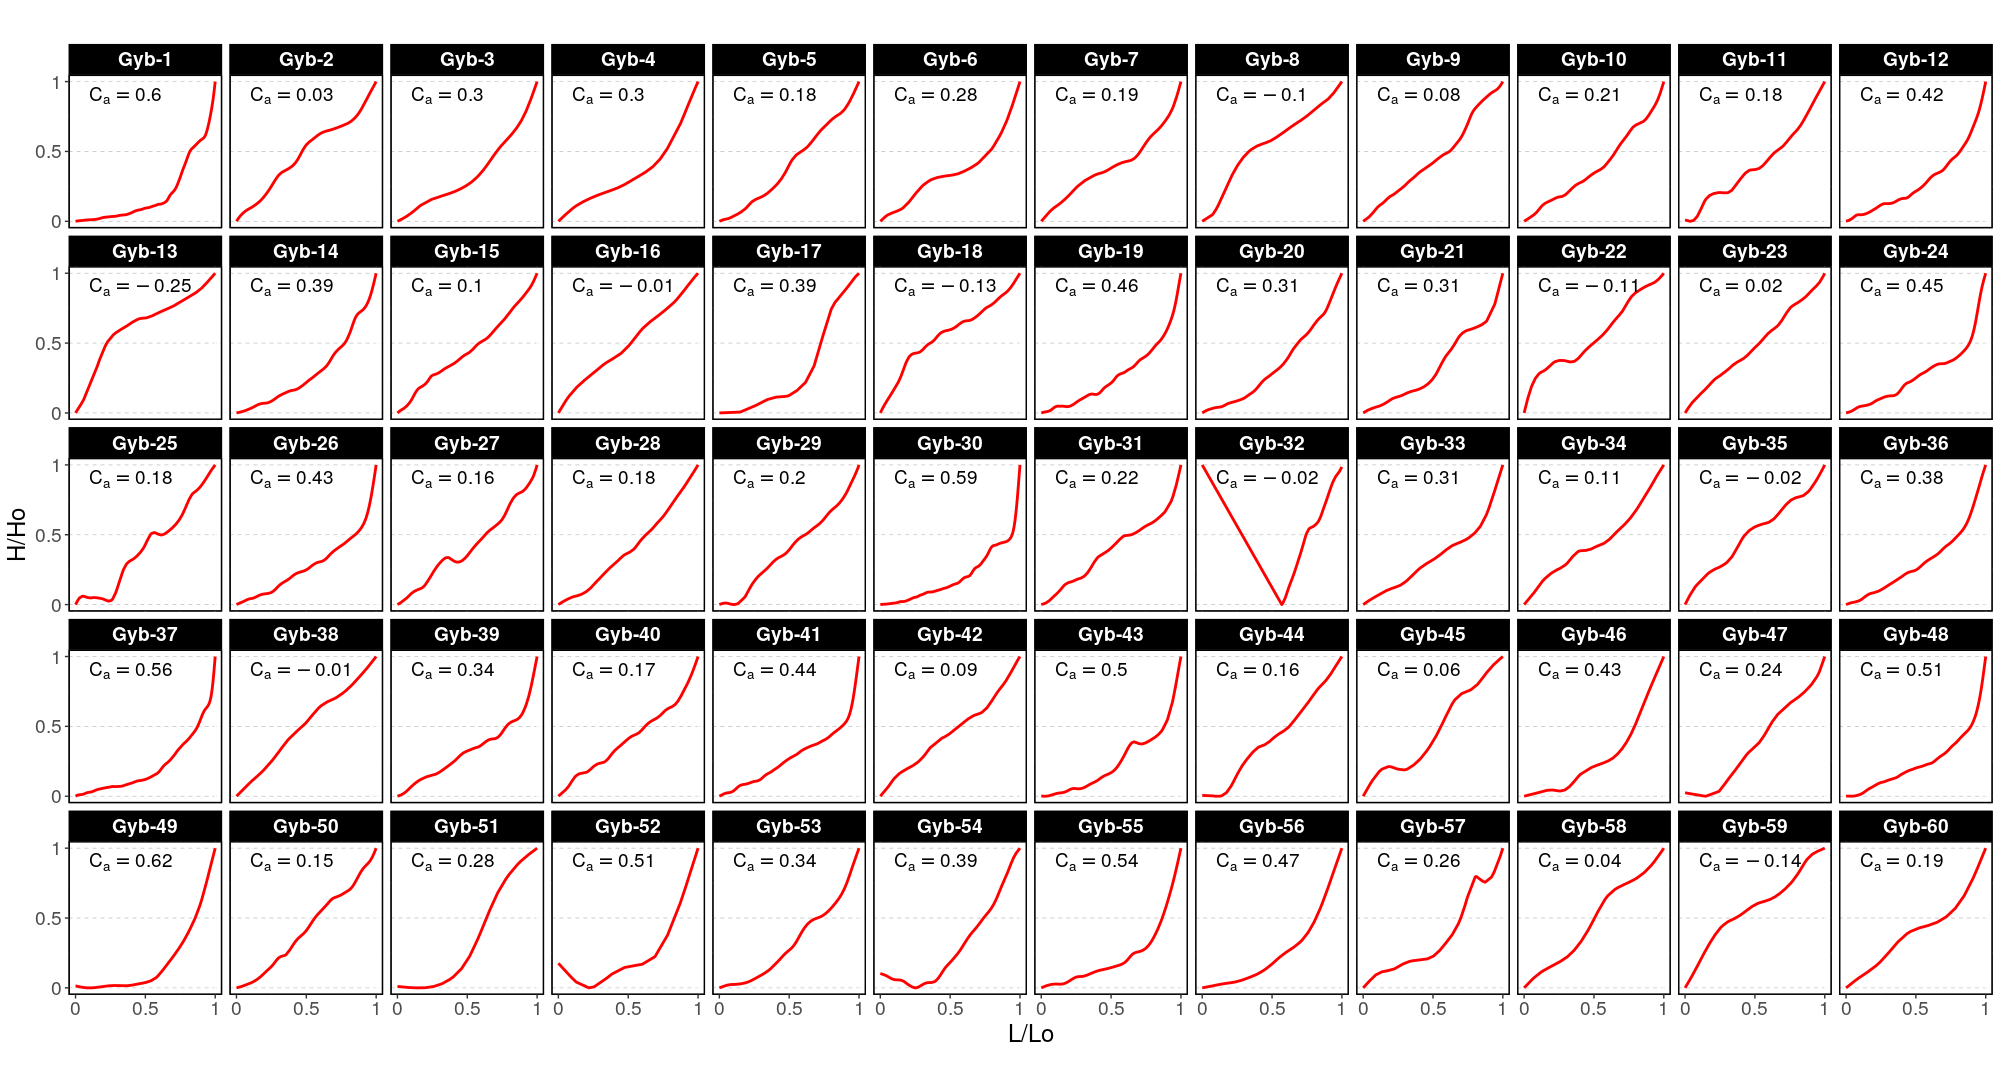
\includegraphics[width=1.00000\textwidth]{Indices de concavidad.png}
\caption{Perfiles longitudinales e índices de concavidad de los cursos
más largos en la cuenca del río Guayubín\label{indicec}}
\end{figure}

\begin{figure}
\centering
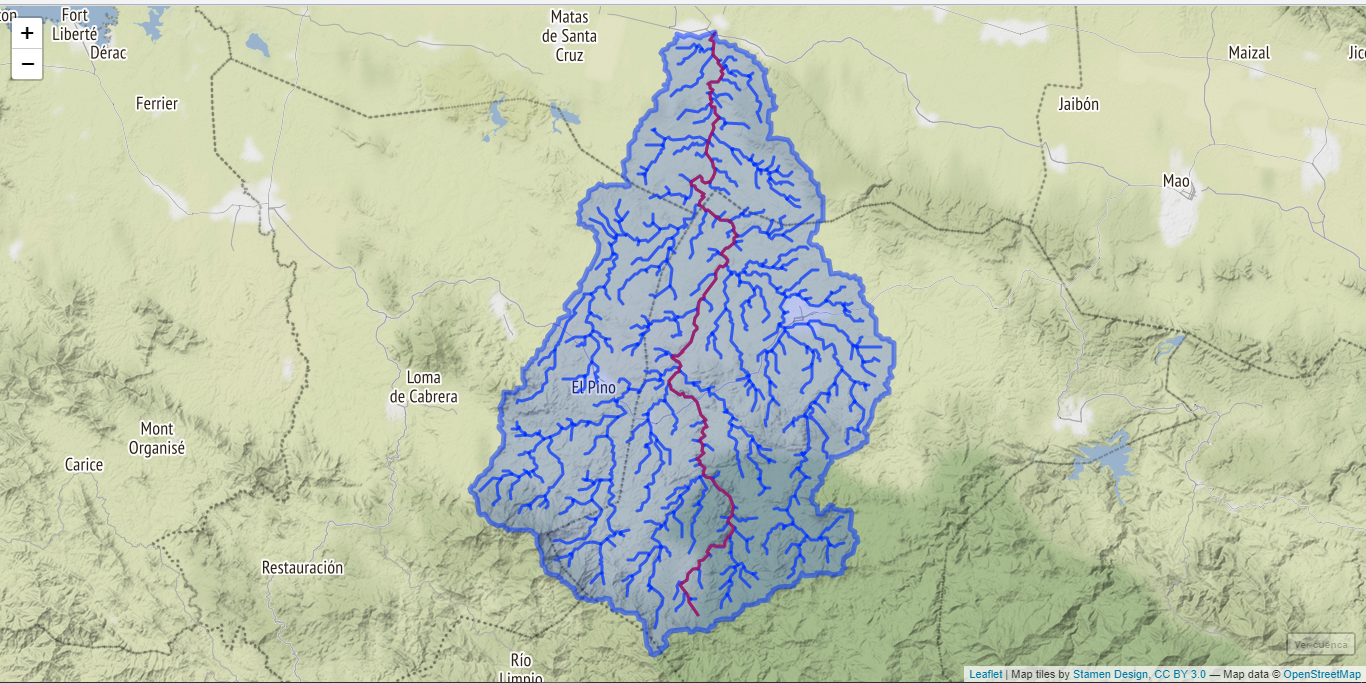
\includegraphics[width=0.60000\textwidth]{cuenca-red de drenaje-curso mas largo.png}
\caption{Cuenca del río Guayubín con su red de drenaje y su curso más
largo\label{vectoresrbasin}}
\end{figure}

\begin{figure}
\centering
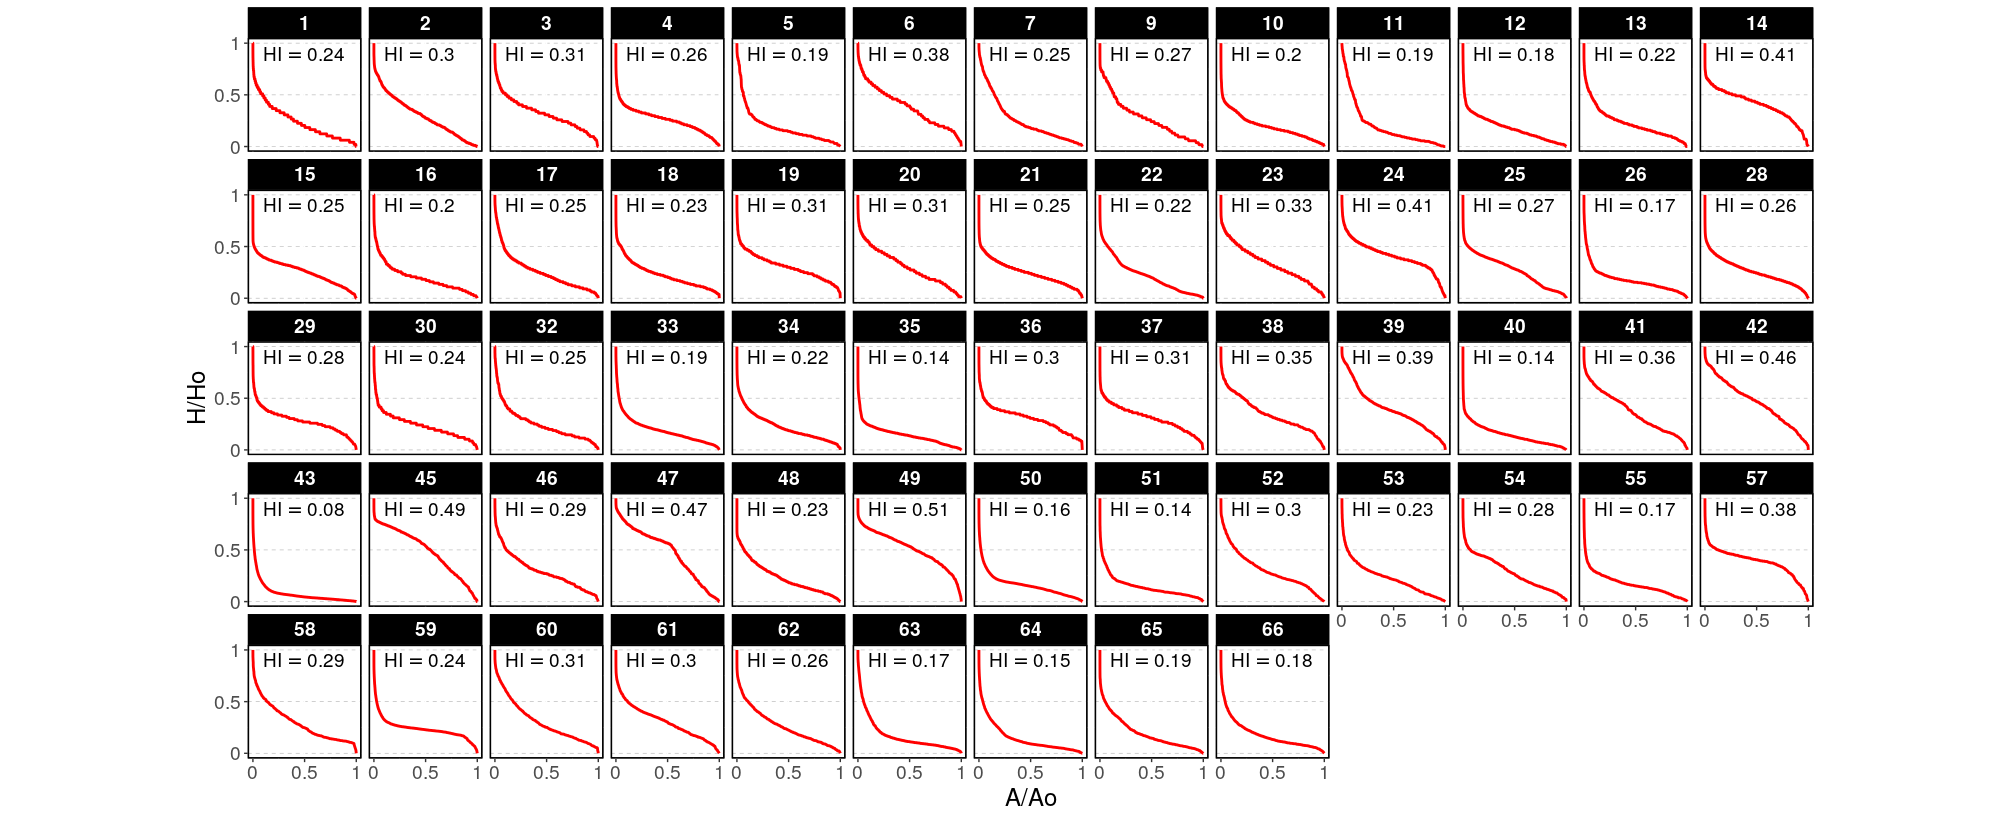
\includegraphics[width=1.10000\textwidth]{HypsoBasinOrder2.png}
\caption{Curva e integral hipsométrica para las cuencas de orden
2\label{hypsob2}}
\end{figure}

\begin{figure}
\centering
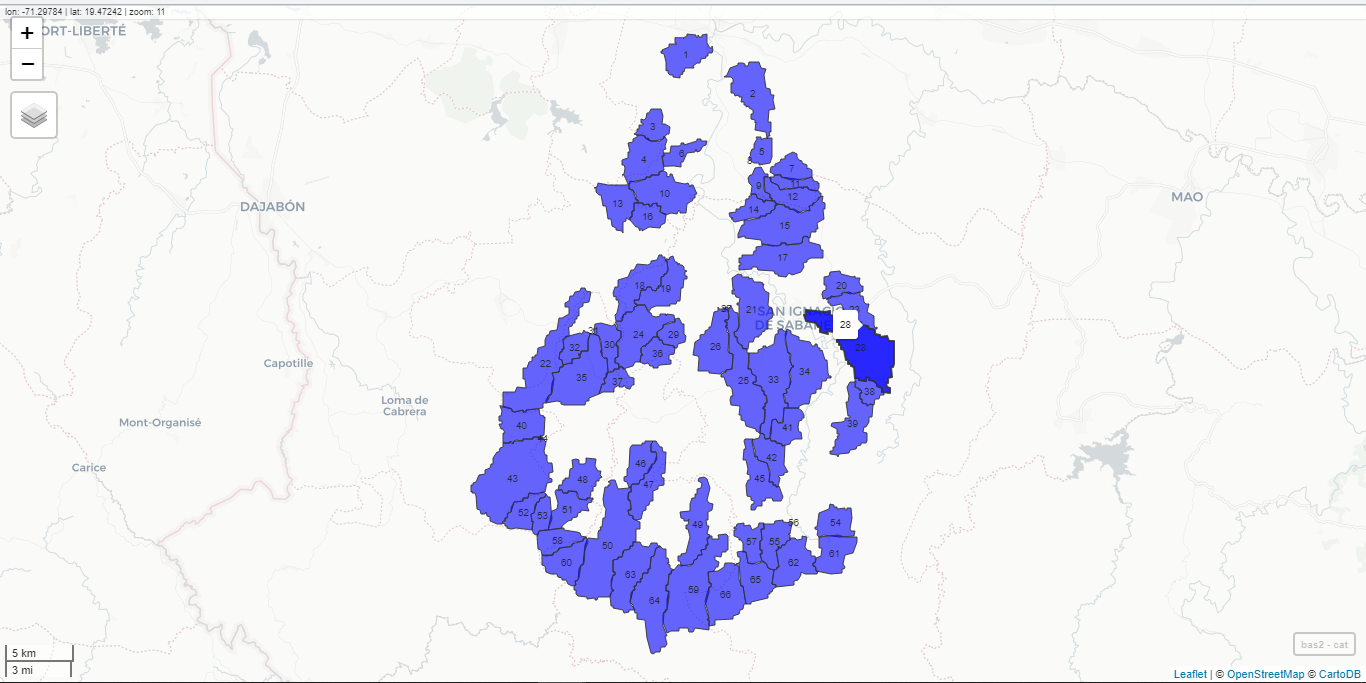
\includegraphics[width=0.90000\textwidth]{Mapview_hypsobasinorder2.png}
\caption{Cuencas de red de drenaje orden 2\label{hypb2}}
\end{figure}

\begin{figure}
\centering
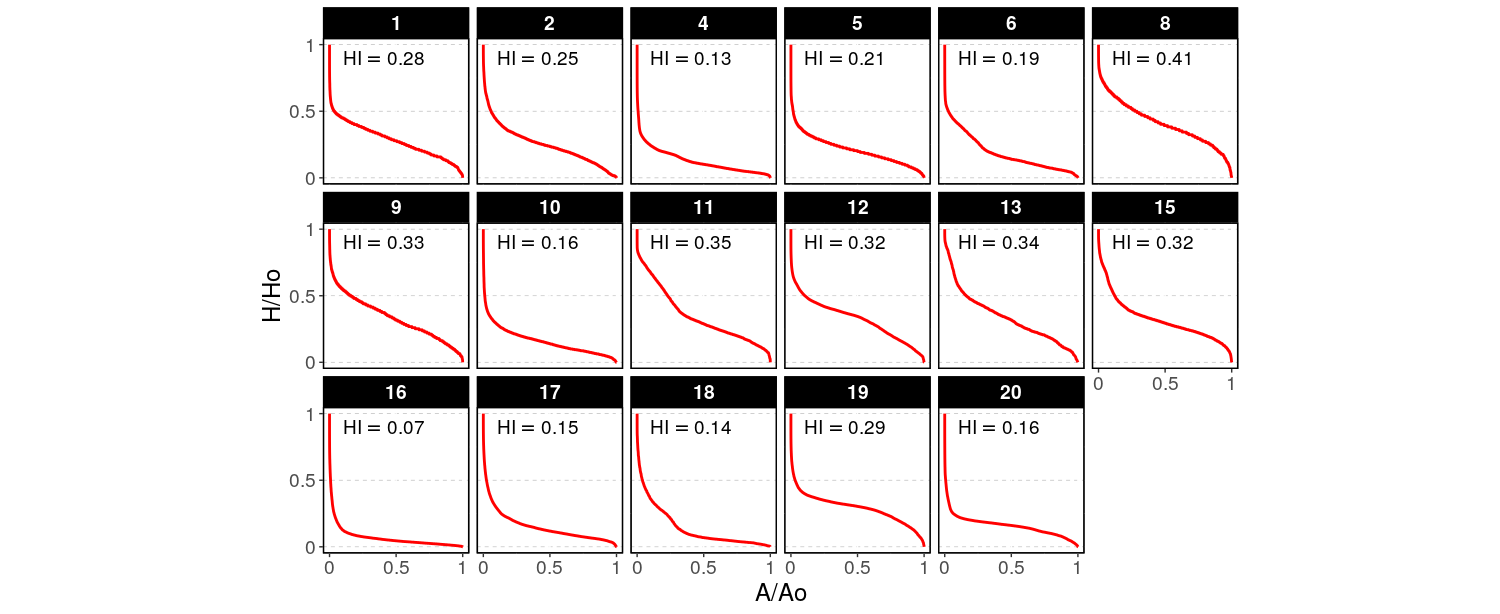
\includegraphics[width=1.00000\textwidth]{HypsoBasinOrder3.png}
\caption{Curva e integral hipsométrica para las cuencas de orden
3\label{hysob3}}
\end{figure}

\begin{figure}
\centering
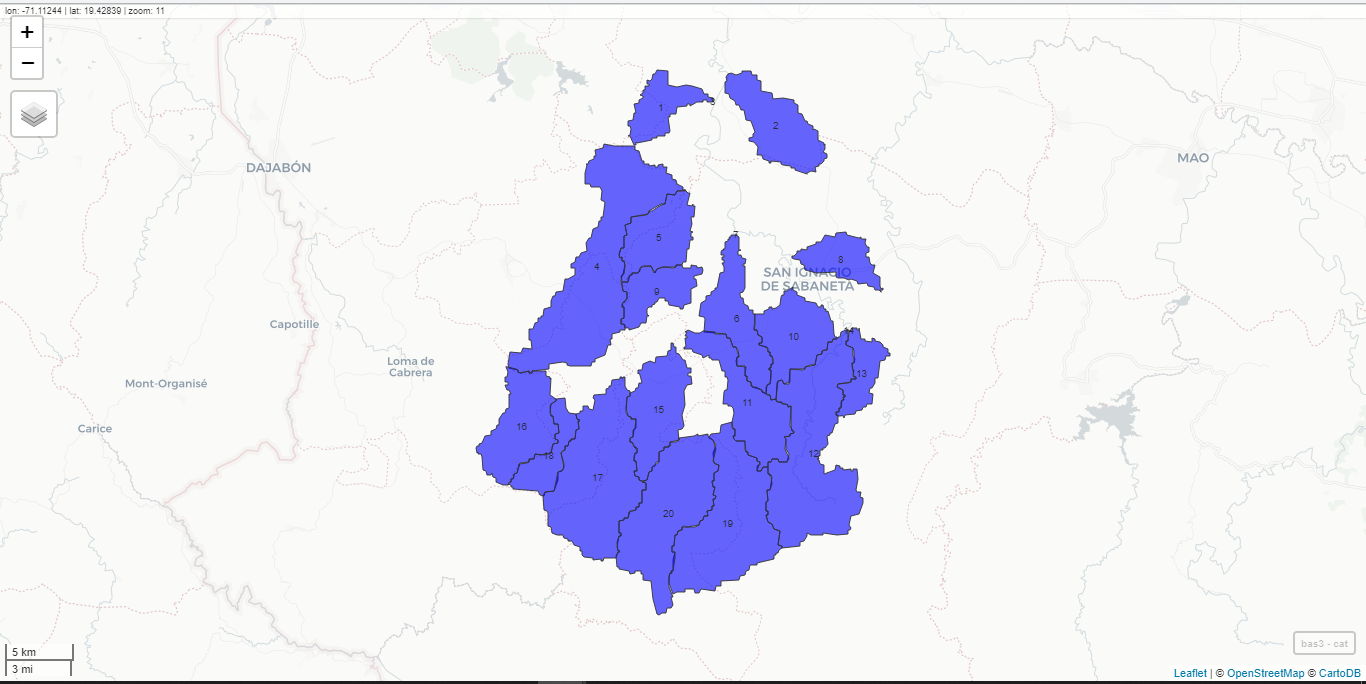
\includegraphics[width=0.90000\textwidth]{Mapview_hypsobasinorder3.png}
\caption{Cuencas de red de drenaje orden 3\label{hypb3}}
\end{figure}

\begin{longtable}[]{@{}cc@{}}
\caption{\label{tab:materiales} Materiales utilizados en la
investigacion.}\tabularnewline
\toprule
\begin{minipage}[b]{0.11\columnwidth}\centering\strut
Materiales\strut
\end{minipage} & \begin{minipage}[b]{0.83\columnwidth}\centering\strut
Uso\strut
\end{minipage}\tabularnewline
\midrule
\endfirsthead
\toprule
\begin{minipage}[b]{0.11\columnwidth}\centering\strut
Materiales\strut
\end{minipage} & \begin{minipage}[b]{0.83\columnwidth}\centering\strut
Uso\strut
\end{minipage}\tabularnewline
\midrule
\endhead
\begin{minipage}[t]{0.11\columnwidth}\centering\strut
RStudio\strut
\end{minipage} & \begin{minipage}[t]{0.83\columnwidth}\centering\strut
Redacción del manuscrito, procesamiento de datos extraídos del \ref{MDE}
de la cuenca a través de un script.\strut
\end{minipage}\tabularnewline
\begin{minipage}[t]{0.11\columnwidth}\centering\strut
library rgrass7\strut
\end{minipage} & \begin{minipage}[t]{0.83\columnwidth}\centering\strut
Creación de interfaz que establecer conexión entre la version 7 del
sistema de infromacion geográfica GRASS y R, que crea un entorno GRASS
desechable dentro de R.\strut
\end{minipage}\tabularnewline
\begin{minipage}[t]{0.11\columnwidth}\centering\strut
library sp\strut
\end{minipage} & \begin{minipage}[t]{0.83\columnwidth}\centering\strut
Importación, manipulación y exportación de datos espaciales en R, e
impresión de los mismos.\strut
\end{minipage}\tabularnewline
\begin{minipage}[t]{0.11\columnwidth}\centering\strut
library sf\strut
\end{minipage} & \begin{minipage}[t]{0.83\columnwidth}\centering\strut
Creación de caracteristicas simples (simple features), que amplían los
objetos tipo data.frame con una columna de lista de características
simples.\strut
\end{minipage}\tabularnewline
\begin{minipage}[t]{0.11\columnwidth}\centering\strut
library raster\strut
\end{minipage} & \begin{minipage}[t]{0.83\columnwidth}\centering\strut
Manipulación de datos geográficos (espaciales) en formato
`ráster'.\strut
\end{minipage}\tabularnewline
\begin{minipage}[t]{0.11\columnwidth}\centering\strut
library leaflet\strut
\end{minipage} & \begin{minipage}[t]{0.83\columnwidth}\centering\strut
Representación de los vectores y rásters.\strut
\end{minipage}\tabularnewline
\begin{minipage}[t]{0.11\columnwidth}\centering\strut
library leafem\strut
\end{minipage} & \begin{minipage}[t]{0.83\columnwidth}\centering\strut
Proveedor de extensión para leaflet usados para paquetes mapview,
permitió mostrar las coordenadas de la posición del puntero del
mouse.\strut
\end{minipage}\tabularnewline
\begin{minipage}[t]{0.11\columnwidth}\centering\strut
library mapview\strut
\end{minipage} & \begin{minipage}[t]{0.83\columnwidth}\centering\strut
Permitió ver los objetos espaciales de forma interactiva.\strut
\end{minipage}\tabularnewline
\begin{minipage}[t]{0.11\columnwidth}\centering\strut
library readr\strut
\end{minipage} & \begin{minipage}[t]{0.83\columnwidth}\centering\strut
Lector de datos rectangulares (como `csv', `tsv' y `fwf').\strut
\end{minipage}\tabularnewline
\begin{minipage}[t]{0.11\columnwidth}\centering\strut
QGIS with GRASS\strut
\end{minipage} & \begin{minipage}[t]{0.83\columnwidth}\centering\strut
Visualizador de vectores y rasters generados con RStudio en una región
de GRASS, de los mapas Topológicos y Geológicos de la República
Dominicana, y, también, Creador de mapas de localización.\strut
\end{minipage}\tabularnewline
\begin{minipage}[t]{0.11\columnwidth}\centering\strut
Google Earth\strut
\end{minipage} & \begin{minipage}[t]{0.83\columnwidth}\centering\strut
Utilizado para observar datos en formato kml generados y exportados de
RStudio y asi como para la representación del relieve del lugar de
estudio.\strut
\end{minipage}\tabularnewline
\begin{minipage}[t]{0.11\columnwidth}\centering\strut
Mapa Topológico de RD\strut
\end{minipage} & \begin{minipage}[t]{0.83\columnwidth}\centering\strut
Mapa para hacer comparaciones y obtener referencias sobre el
relieve.\strut
\end{minipage}\tabularnewline
\begin{minipage}[t]{0.11\columnwidth}\centering\strut
Mapa Geológico Nacional de RD\strut
\end{minipage} & \begin{minipage}[t]{0.83\columnwidth}\centering\strut
Mapa para hacer comparaciones y obtener referencias sobre la composición
rocosa y los años que datan estas (ver figura\ref{magecu}).\strut
\end{minipage}\tabularnewline
\bottomrule
\end{longtable}

\begin{longtable}[]{@{}cccccc@{}}
\caption{\label{tab:estadisticaor} Estadisticas de los ordenes de red
del rio Guayubin}\tabularnewline
\toprule
Max order & Tot.N.str. & Tot.str.len. & Tot.area. & Dr.dens. &
Str.freq.\tabularnewline
\midrule
\endfirsthead
\toprule
Max order & Tot.N.str. & Tot.str.len. & Tot.area. & Dr.dens. &
Str.freq.\tabularnewline
\midrule
\endhead
(num) & (num) & (km) & (km\textsuperscript{2}) &
(km/km\textsuperscript{2}) & (num/km\textsuperscript{2})\tabularnewline
5 & 367 & 693.6069 & 773.2235 & 0.8970 & 0.4746\tabularnewline
\bottomrule
\end{longtable}

\begin{longtable}[]{@{}ccccc@{}}
\caption{\label{tab:regresionc} Razones de cursos basados en el
coeficiente de regresion}\tabularnewline
\toprule
Bif.rt. & Len.rt. & Area.rt. & Slo.rt. & Grd.rt.\tabularnewline
\midrule
\endfirsthead
\toprule
Bif.rt. & Len.rt. & Area.rt. & Slo.rt. & Grd.rt.\tabularnewline
\midrule
\endhead
4.0643 & 2.2928 & 4.5845 & 1.4798 & 1.8338\tabularnewline
\bottomrule
\end{longtable}

\begin{longtable}[]{@{}ccccc@{}}
\caption{\label{estandard} Relaciones de flujo promediadas con
desviaciones estándar}\tabularnewline
\toprule
Bif.rt. & Len.rt. & Area.rt. & Slo.rt. & Grd.rt.\tabularnewline
\midrule
\endfirsthead
\toprule
Bif.rt. & Len.rt. & Area.rt. & Slo.rt. & Grd.rt.\tabularnewline
\midrule
\endhead
4.1235 & 2.3822 & 3.3126 & 1.4938 & 1.9010\tabularnewline
0.4476 & 0.6025 & 2.2153 & 0.0960 & 0.5050\tabularnewline
\bottomrule
\end{longtable}

\begin{longtable}[]{@{}cccccc@{}}
\caption{\label{promo} Variables promediadas para cada orden de
red}\tabularnewline
\toprule
\begin{minipage}[b]{0.08\columnwidth}\centering\strut
Order num\strut
\end{minipage} & \begin{minipage}[b]{0.11\columnwidth}\centering\strut
Avg.len (km)\strut
\end{minipage} & \begin{minipage}[b]{0.25\columnwidth}\centering\strut
Avg.ar (km\textsuperscript{2})\strut
\end{minipage} & \begin{minipage}[b]{0.11\columnwidth}\centering\strut
Avg.sl (m/m)\strut
\end{minipage} & \begin{minipage}[b]{0.14\columnwidth}\centering\strut
Avg.grad. (m/m)\strut
\end{minipage} & \begin{minipage}[b]{0.13\columnwidth}\centering\strut
Avg.el.dif (m)\strut
\end{minipage}\tabularnewline
\midrule
\endfirsthead
\toprule
\begin{minipage}[b]{0.08\columnwidth}\centering\strut
Order num\strut
\end{minipage} & \begin{minipage}[b]{0.11\columnwidth}\centering\strut
Avg.len (km)\strut
\end{minipage} & \begin{minipage}[b]{0.25\columnwidth}\centering\strut
Avg.ar (km\textsuperscript{2})\strut
\end{minipage} & \begin{minipage}[b]{0.11\columnwidth}\centering\strut
Avg.sl (m/m)\strut
\end{minipage} & \begin{minipage}[b]{0.14\columnwidth}\centering\strut
Avg.grad. (m/m)\strut
\end{minipage} & \begin{minipage}[b]{0.13\columnwidth}\centering\strut
Avg.el.dif (m)\strut
\end{minipage}\tabularnewline
\midrule
\endhead
\begin{minipage}[t]{0.08\columnwidth}\centering\strut
1\strut
\end{minipage} & \begin{minipage}[t]{0.11\columnwidth}\centering\strut
1.2435\strut
\end{minipage} & \begin{minipage}[t]{0.25\columnwidth}\centering\strut
1.7188\strut
\end{minipage} & \begin{minipage}[t]{0.11\columnwidth}\centering\strut
0.0367\strut
\end{minipage} & \begin{minipage}[t]{0.14\columnwidth}\centering\strut
0.0296\strut
\end{minipage} & \begin{minipage}[t]{0.13\columnwidth}\centering\strut
37.4437\strut
\end{minipage}\tabularnewline
\begin{minipage}[t]{0.08\columnwidth}\centering\strut
2\strut
\end{minipage} & \begin{minipage}[t]{0.11\columnwidth}\centering\strut
2.4743\strut
\end{minipage} & \begin{minipage}[t]{0.25\columnwidth}\centering\strut
7.2904\strut
\end{minipage} & \begin{minipage}[t]{0.11\columnwidth}\centering\strut
0.0246\strut
\end{minipage} & \begin{minipage}[t]{0.14\columnwidth}\centering\strut
0.0201\strut
\end{minipage} & \begin{minipage}[t]{0.13\columnwidth}\centering\strut
49.0820\strut
\end{minipage}\tabularnewline
\begin{minipage}[t]{0.08\columnwidth}\centering\strut
3\strut
\end{minipage} & \begin{minipage}[t]{0.11\columnwidth}\centering\strut
6.2881\strut
\end{minipage} & \begin{minipage}[t]{0.25\columnwidth}\centering\strut
31.7328\strut
\end{minipage} & \begin{minipage}[t]{0.11\columnwidth}\centering\strut
0.0165\strut
\end{minipage} & \begin{minipage}[t]{0.14\columnwidth}\centering\strut
0.0113\strut
\end{minipage} & \begin{minipage}[t]{0.13\columnwidth}\centering\strut
85.1765\strut
\end{minipage}\tabularnewline
\begin{minipage}[t]{0.08\columnwidth}\centering\strut
4\strut
\end{minipage} & \begin{minipage}[t]{0.11\columnwidth}\centering\strut
11.5356\strut
\end{minipage} & \begin{minipage}[t]{0.25\columnwidth}\centering\strut
147.7492\strut
\end{minipage} & \begin{minipage}[t]{0.11\columnwidth}\centering\strut
0.0120\strut
\end{minipage} & \begin{minipage}[t]{0.14\columnwidth}\centering\strut
0.0066\strut
\end{minipage} & \begin{minipage}[t]{0.13\columnwidth}\centering\strut
80.0000\strut
\end{minipage}\tabularnewline
\begin{minipage}[t]{0.08\columnwidth}\centering\strut
5\strut
\end{minipage} & \begin{minipage}[t]{0.11\columnwidth}\centering\strut
36.4888\strut
\end{minipage} & \begin{minipage}[t]{0.25\columnwidth}\centering\strut
773.2235\strut
\end{minipage} & \begin{minipage}[t]{0.11\columnwidth}\centering\strut
0.0074\strut
\end{minipage} & \begin{minipage}[t]{0.14\columnwidth}\centering\strut
0.0025\strut
\end{minipage} & \begin{minipage}[t]{0.13\columnwidth}\centering\strut
91.0000\strut
\end{minipage}\tabularnewline
\bottomrule
\end{longtable}

\begin{longtable}[]{@{}cccccc@{}}
\caption{\label{estad} Desviacion estandar para las estadisticas segun
orden de red}\tabularnewline
\toprule
\begin{minipage}[b]{0.08\columnwidth}\centering\strut
Order num\strut
\end{minipage} & \begin{minipage}[b]{0.11\columnwidth}\centering\strut
Std.len (km)\strut
\end{minipage} & \begin{minipage}[b]{0.26\columnwidth}\centering\strut
Std.ar (km\textsuperscript{2})\strut
\end{minipage} & \begin{minipage}[b]{0.11\columnwidth}\centering\strut
Std.sl (m/m)\strut
\end{minipage} & \begin{minipage}[b]{0.14\columnwidth}\centering\strut
Std.grad. (m/m)\strut
\end{minipage} & \begin{minipage}[b]{0.13\columnwidth}\centering\strut
Std.el.dif (m)\strut
\end{minipage}\tabularnewline
\midrule
\endfirsthead
\toprule
\begin{minipage}[b]{0.08\columnwidth}\centering\strut
Order num\strut
\end{minipage} & \begin{minipage}[b]{0.11\columnwidth}\centering\strut
Std.len (km)\strut
\end{minipage} & \begin{minipage}[b]{0.26\columnwidth}\centering\strut
Std.ar (km\textsuperscript{2})\strut
\end{minipage} & \begin{minipage}[b]{0.11\columnwidth}\centering\strut
Std.sl (m/m)\strut
\end{minipage} & \begin{minipage}[b]{0.14\columnwidth}\centering\strut
Std.grad. (m/m)\strut
\end{minipage} & \begin{minipage}[b]{0.13\columnwidth}\centering\strut
Std.el.dif (m)\strut
\end{minipage}\tabularnewline
\midrule
\endhead
\begin{minipage}[t]{0.08\columnwidth}\centering\strut
1\strut
\end{minipage} & \begin{minipage}[t]{0.11\columnwidth}\centering\strut
1.0274\strut
\end{minipage} & \begin{minipage}[t]{0.26\columnwidth}\centering\strut
1.0955\strut
\end{minipage} & \begin{minipage}[t]{0.11\columnwidth}\centering\strut
0.0379\strut
\end{minipage} & \begin{minipage}[t]{0.14\columnwidth}\centering\strut
0.0324\strut
\end{minipage} & \begin{minipage}[t]{0.13\columnwidth}\centering\strut
52.7742\strut
\end{minipage}\tabularnewline
\begin{minipage}[t]{0.08\columnwidth}\centering\strut
2\strut
\end{minipage} & \begin{minipage}[t]{0.11\columnwidth}\centering\strut
1.9695\strut
\end{minipage} & \begin{minipage}[t]{0.26\columnwidth}\centering\strut
4.4097\strut
\end{minipage} & \begin{minipage}[t]{0.11\columnwidth}\centering\strut
0.0215\strut
\end{minipage} & \begin{minipage}[t]{0.14\columnwidth}\centering\strut
0.0194\strut
\end{minipage} & \begin{minipage}[t]{0.13\columnwidth}\centering\strut
52.5830\strut
\end{minipage}\tabularnewline
\begin{minipage}[t]{0.08\columnwidth}\centering\strut
3\strut
\end{minipage} & \begin{minipage}[t]{0.11\columnwidth}\centering\strut
5.0992\strut
\end{minipage} & \begin{minipage}[t]{0.26\columnwidth}\centering\strut
19.0637\strut
\end{minipage} & \begin{minipage}[t]{0.11\columnwidth}\centering\strut
0.0092\strut
\end{minipage} & \begin{minipage}[t]{0.14\columnwidth}\centering\strut
0.0077\strut
\end{minipage} & \begin{minipage}[t]{0.13\columnwidth}\centering\strut
93.4085\strut
\end{minipage}\tabularnewline
\begin{minipage}[t]{0.08\columnwidth}\centering\strut
4\strut
\end{minipage} & \begin{minipage}[t]{0.11\columnwidth}\centering\strut
5.8247\strut
\end{minipage} & \begin{minipage}[t]{0.26\columnwidth}\centering\strut
44.3177\strut
\end{minipage} & \begin{minipage}[t]{0.11\columnwidth}\centering\strut
0.0041\strut
\end{minipage} & \begin{minipage}[t]{0.14\columnwidth}\centering\strut
0.0032\strut
\end{minipage} & \begin{minipage}[t]{0.13\columnwidth}\centering\strut
57.0789\strut
\end{minipage}\tabularnewline
\begin{minipage}[t]{0.08\columnwidth}\centering\strut
5\strut
\end{minipage} & \begin{minipage}[t]{0.11\columnwidth}\centering\strut
-0.0000\strut
\end{minipage} & \begin{minipage}[t]{0.26\columnwidth}\centering\strut
0.0000\strut
\end{minipage} & \begin{minipage}[t]{0.11\columnwidth}\centering\strut
0.0000\strut
\end{minipage} & \begin{minipage}[t]{0.14\columnwidth}\centering\strut
0.0000\strut
\end{minipage} & \begin{minipage}[t]{0.13\columnwidth}\centering\strut
0.0000\strut
\end{minipage}\tabularnewline
\bottomrule
\end{longtable}

\begin{longtable}[]{@{}cccc@{}}
\caption{\label{parh} Estadisticas de parametros hidrgograficos segun el
orden de red}\tabularnewline
\toprule
Order & N.streams & Tot.len (km) & Tot.area
(km\textsuperscript{2})\tabularnewline
\midrule
\endfirsthead
\toprule
Order & N.streams & Tot.len (km) & Tot.area
(km\textsuperscript{2})\tabularnewline
\midrule
\endhead
1 & 284 & 353.1463 & 488.1383\tabularnewline
2 & 61 & 150.9325 & 444.7173\tabularnewline
3 & 17 & 106.8969 & 539.4576\tabularnewline
4 & 4 & 46.1425 & 590.9969\tabularnewline
5 & 1 & 36.4888 & 773.2235\tabularnewline
\bottomrule
\end{longtable}

\begin{longtable}[]{@{}cccccccc@{}}
\caption{\label{razones} Razones de los parametros hidrograficos segun
su orden de red}\tabularnewline
\toprule
Order & Bif.rt. & Len.rt. & Area.rt. & Slo.rt. & Grd.rt. & d.dens. &
str.freq.\tabularnewline
\midrule
\endfirsthead
\toprule
Order & Bif.rt. & Len.rt. & Area.rt. & Slo.rt. & Grd.rt. & d.dens. &
str.freq.\tabularnewline
\midrule
\endhead
1 & 4.6557 & 1.9898 & 0.0000 & 1.4930 & 1.4748 & 0.7235 &
0.5818\tabularnewline
2 & 3.5882 & 2.5413 & 4.2416 & 1.4930 & 1.7757 & 0.3394 &
0.1372\tabularnewline
3 & 4.2500 & 1.8345 & 4.3527 & 1.3771 & 1.7207 & 0.1982 &
0.0315\tabularnewline
4 & 4.0000 & 3.1631 & 4.6560 & 1.6122 & 2.6327 & 0.0781 &
0.0068\tabularnewline
5 & 0.0000 & 0.0000 & 5.2334 & 0.0000 & 0.0000 & 0.0472 &
0.0013\tabularnewline
\bottomrule
\end{longtable}

\begin{longtable}[]{@{}cc@{}}
\caption{\label{tab:parametrosm}Parámetros morfométricos de la cuenca
del río Guayubín.}\tabularnewline
\toprule
\begin{minipage}[b]{0.65\columnwidth}\centering\strut
Parámetros\strut
\end{minipage} & \begin{minipage}[b]{0.29\columnwidth}\centering\strut
Valores\strut
\end{minipage}\tabularnewline
\midrule
\endfirsthead
\toprule
\begin{minipage}[b]{0.65\columnwidth}\centering\strut
Parámetros\strut
\end{minipage} & \begin{minipage}[b]{0.29\columnwidth}\centering\strut
Valores\strut
\end{minipage}\tabularnewline
\midrule
\endhead
\begin{minipage}[t]{0.65\columnwidth}\centering\strut
Easting Centroid of basin\strut
\end{minipage} & \begin{minipage}[t]{0.29\columnwidth}\centering\strut
246465.00\strut
\end{minipage}\tabularnewline
\begin{minipage}[t]{0.65\columnwidth}\centering\strut
Northing Centroid of basin\strut
\end{minipage} & \begin{minipage}[t]{0.29\columnwidth}\centering\strut
2151675.00\strut
\end{minipage}\tabularnewline
\begin{minipage}[t]{0.65\columnwidth}\centering\strut
Rectangle containing basin N-W\strut
\end{minipage} & \begin{minipage}[t]{0.29\columnwidth}\centering\strut
(`230220', `2175930')\strut
\end{minipage}\tabularnewline
\begin{minipage}[t]{0.65\columnwidth}\centering\strut
Rectangle containing basin S-E\strut
\end{minipage} & \begin{minipage}[t]{0.29\columnwidth}\centering\strut
(`261000', `2131290')\strut
\end{minipage}\tabularnewline
\begin{minipage}[t]{0.65\columnwidth}\centering\strut
Area of basin {[}km\textsuperscript{2}{]}\strut
\end{minipage} & \begin{minipage}[t]{0.29\columnwidth}\centering\strut
773.5631625\strut
\end{minipage}\tabularnewline
\begin{minipage}[t]{0.65\columnwidth}\centering\strut
Perimeter of basin {[}km{]}\strut
\end{minipage} & \begin{minipage}[t]{0.29\columnwidth}\centering\strut
156.122652506552\strut
\end{minipage}\tabularnewline
\begin{minipage}[t]{0.65\columnwidth}\centering\strut
Max Elevation {[}m s.l.m.{]}\strut
\end{minipage} & \begin{minipage}[t]{0.29\columnwidth}\centering\strut
1396.72540740785\strut
\end{minipage}\tabularnewline
\begin{minipage}[t]{0.65\columnwidth}\centering\strut
Min Elevation {[}m s.l.m.{]}\strut
\end{minipage} & \begin{minipage}[t]{0.29\columnwidth}\centering\strut
30.9651954818271\strut
\end{minipage}\tabularnewline
\begin{minipage}[t]{0.65\columnwidth}\centering\strut
Elevation Difference {[}m{]}\strut
\end{minipage} & \begin{minipage}[t]{0.29\columnwidth}\centering\strut
1365.760211926023\strut
\end{minipage}\tabularnewline
\begin{minipage}[t]{0.65\columnwidth}\centering\strut
Mean Elevation\strut
\end{minipage} & \begin{minipage}[t]{0.29\columnwidth}\centering\strut
276.7019\strut
\end{minipage}\tabularnewline
\begin{minipage}[t]{0.65\columnwidth}\centering\strut
Mean Slope\strut
\end{minipage} & \begin{minipage}[t]{0.29\columnwidth}\centering\strut
5.17\strut
\end{minipage}\tabularnewline
\begin{minipage}[t]{0.65\columnwidth}\centering\strut
Length of Directing Vector {[}km{]}\strut
\end{minipage} & \begin{minipage}[t]{0.29\columnwidth}\centering\strut
24.460893544594807\strut
\end{minipage}\tabularnewline
\begin{minipage}[t]{0.65\columnwidth}\centering\strut
Prevalent Orientation {[}degree from north, counterclockwise{]}\strut
\end{minipage} & \begin{minipage}[t]{0.29\columnwidth}\centering\strut
1.4935760627096282\strut
\end{minipage}\tabularnewline
\begin{minipage}[t]{0.65\columnwidth}\centering\strut
Compactness Coefficient\strut
\end{minipage} & \begin{minipage}[t]{0.29\columnwidth}\centering\strut
4.974655054098116\strut
\end{minipage}\tabularnewline
\begin{minipage}[t]{0.65\columnwidth}\centering\strut
Circularity Ratio\strut
\end{minipage} & \begin{minipage}[t]{0.29\columnwidth}\centering\strut
0.3988171279899944\strut
\end{minipage}\tabularnewline
\begin{minipage}[t]{0.65\columnwidth}\centering\strut
Topological Diameter\strut
\end{minipage} & \begin{minipage}[t]{0.29\columnwidth}\centering\strut
84.0\strut
\end{minipage}\tabularnewline
\begin{minipage}[t]{0.65\columnwidth}\centering\strut
Elongation Ratio\strut
\end{minipage} & \begin{minipage}[t]{0.29\columnwidth}\centering\strut
0.5064682945330589\strut
\end{minipage}\tabularnewline
\begin{minipage}[t]{0.65\columnwidth}\centering\strut
Shape Factor\strut
\end{minipage} & \begin{minipage}[t]{0.29\columnwidth}\centering\strut
12.483750895456415\strut
\end{minipage}\tabularnewline
\begin{minipage}[t]{0.65\columnwidth}\centering\strut
Concentration Time (Giandotti, 1934) {[}hr{]}\strut
\end{minipage} & \begin{minipage}[t]{0.29\columnwidth}\centering\strut
6.906840311938352\strut
\end{minipage}\tabularnewline
\begin{minipage}[t]{0.65\columnwidth}\centering\strut
Length of Mainchannel {[}km{]}\strut
\end{minipage} & \begin{minipage}[t]{0.29\columnwidth}\centering\strut
61.965603846\strut
\end{minipage}\tabularnewline
\begin{minipage}[t]{0.65\columnwidth}\centering\strut
Mean slope of mainchannel {[}percent{]}\strut
\end{minipage} & \begin{minipage}[t]{0.29\columnwidth}\centering\strut
1.9669190473941982\strut
\end{minipage}\tabularnewline
\begin{minipage}[t]{0.65\columnwidth}\centering\strut
Mean hillslope length {[}m{]}\strut
\end{minipage} & \begin{minipage}[t]{0.29\columnwidth}\centering\strut
250.4986\strut
\end{minipage}\tabularnewline
\begin{minipage}[t]{0.65\columnwidth}\centering\strut
Magnitudo\strut
\end{minipage} & \begin{minipage}[t]{0.29\columnwidth}\centering\strut
223.0\strut
\end{minipage}\tabularnewline
\begin{minipage}[t]{0.65\columnwidth}\centering\strut
Max order (Strahler)\strut
\end{minipage} & \begin{minipage}[t]{0.29\columnwidth}\centering\strut
5\strut
\end{minipage}\tabularnewline
\begin{minipage}[t]{0.65\columnwidth}\centering\strut
Number of streams\strut
\end{minipage} & \begin{minipage}[t]{0.29\columnwidth}\centering\strut
343\strut
\end{minipage}\tabularnewline
\begin{minipage}[t]{0.65\columnwidth}\centering\strut
Total Stream Length {[}km{]}\strut
\end{minipage} & \begin{minipage}[t]{0.29\columnwidth}\centering\strut
662.2185\strut
\end{minipage}\tabularnewline
\begin{minipage}[t]{0.65\columnwidth}\centering\strut
First order stream frequency\strut
\end{minipage} & \begin{minipage}[t]{0.29\columnwidth}\centering\strut
0.2882763952710843\strut
\end{minipage}\tabularnewline
\begin{minipage}[t]{0.65\columnwidth}\centering\strut
Drainage Density {[}km/km\textsuperscript{2}{]}\strut
\end{minipage} & \begin{minipage}[t]{0.29\columnwidth}\centering\strut
0.8560626101427108\strut
\end{minipage}\tabularnewline
\begin{minipage}[t]{0.65\columnwidth}\centering\strut
Bifurcation Ratio (Horton)\strut
\end{minipage} & \begin{minipage}[t]{0.29\columnwidth}\centering\strut
3.8876\strut
\end{minipage}\tabularnewline
\begin{minipage}[t]{0.65\columnwidth}\centering\strut
Length Ratio (Horton)\strut
\end{minipage} & \begin{minipage}[t]{0.29\columnwidth}\centering\strut
2.2966\strut
\end{minipage}\tabularnewline
\begin{minipage}[t]{0.65\columnwidth}\centering\strut
Area ratio (Horton)\strut
\end{minipage} & \begin{minipage}[t]{0.29\columnwidth}\centering\strut
4.3704\strut
\end{minipage}\tabularnewline
\begin{minipage}[t]{0.65\columnwidth}\centering\strut
Slope ratio (Horton)\strut
\end{minipage} & \begin{minipage}[t]{0.29\columnwidth}\centering\strut
1.4689\strut
\end{minipage}\tabularnewline
\bottomrule
\end{longtable}

\begin{longtable}[]{@{}cc@{}}
\caption{\label{ihco2} Integral hipsométrica en las cuencas de orden
2}\tabularnewline
\toprule
Categoría & Integral hipsométrica\tabularnewline
\midrule
\endfirsthead
\toprule
Categoría & Integral hipsométrica\tabularnewline
\midrule
\endhead
1 & 0.23784092\tabularnewline
2 & 0.29691935\tabularnewline
3 & 0.31478851\tabularnewline
4 & 0.25845620\tabularnewline
5 & 0.18914104\tabularnewline
6 & 0.38449116\tabularnewline
7 & 0.25087104\tabularnewline
9 & 0.26943542\tabularnewline
10 & 0.19779399\tabularnewline
11 & 0.19287436\tabularnewline
12 & 0.17808813\tabularnewline
13 & 0.22437828\tabularnewline
14 & 0.40595651\tabularnewline
15 & 0.25477715\tabularnewline
16 & 0.19777159\tabularnewline
17 & 0.25313336\tabularnewline
18 & 0.22679929\tabularnewline
19 & 0.30597060\tabularnewline
20 & 0.30564285\tabularnewline
21 & 0.24773997\tabularnewline
22 & 0.21800099\tabularnewline
23 & 0.33229314\tabularnewline
24 & 0.40758028\tabularnewline
25 & 0.27096759\tabularnewline
26 & 0.17485732\tabularnewline
28 & 0.25721054\tabularnewline
29 & 0.27907973\tabularnewline
30 & 0.23545394\tabularnewline
32 & 0.24544610\tabularnewline
33 & 0.18990261\tabularnewline
34 & 0.22303577\tabularnewline
35 & 0.14436574\tabularnewline
36 & 0.30229714\tabularnewline
37 & 0.30742281\tabularnewline
38 & 0.34876647\tabularnewline
39 & 0.39371293\tabularnewline
40 & 0.14419677\tabularnewline
41 & 0.36397062\tabularnewline
42 & 0.45795809\tabularnewline
43 & 0.07642614\tabularnewline
45 & 0.48672629\tabularnewline
46 & 0.29182502\tabularnewline
47 & 0.47300056\tabularnewline
48 & 0.22892086\tabularnewline
49 & 0.50910119\tabularnewline
50 & 0.16011357\tabularnewline
51 & 0.14325914\tabularnewline
52 & 0.30243670\tabularnewline
53 & 0.22622911\tabularnewline
54 & 0.27985062\tabularnewline
55 & 0.16980308\tabularnewline
57 & 0.38363564\tabularnewline
58 & 0.29000326\tabularnewline
59 & 0.23691203\tabularnewline
60 & 0.30564446\tabularnewline
61 & 0.30401039\tabularnewline
62 & 0.25939942\tabularnewline
63 & 0.16711030\tabularnewline
64 & 0.14693431\tabularnewline
65 & 0.19359746\tabularnewline
66 & 0.17854689\tabularnewline
\bottomrule
\end{longtable}

\begin{longtable}[]{@{}cc@{}}
\caption{\label{ihco3} Integral hipsométrica en las cuencas de orden
3}\tabularnewline
\toprule
Categoría & Integral hipsométrico\tabularnewline
\midrule
\endfirsthead
\toprule
Categoría & Integral hipsométrico\tabularnewline
\midrule
\endhead
1 & 0.28106607\tabularnewline
2 & 0.24855493\tabularnewline
4 & 0.12697883\tabularnewline
5 & 0.21021494\tabularnewline
6 & 0.18586633\tabularnewline
8 & 0.40849637\tabularnewline
9 & 0.33264116\tabularnewline
10 & 0.15880640\tabularnewline
11 & 0.34507681\tabularnewline
12 & 0.32371339\tabularnewline
13 & 0.33707592\tabularnewline
15 & 0.32319904\tabularnewline
16 & 0.06673204\tabularnewline
17 & 0.15091492\tabularnewline
18 & 0.14111015\tabularnewline
19 & 0.29051932\tabularnewline
20 & 0.15859746\tabularnewline
\bottomrule
\end{longtable}

\section{\texorpdfstring{\emph{Script}
reproducible}{Script reproducible}}\label{script-reproducible}

\section*{Referencia}\label{referencia}
\addcontentsline{toc}{section}{Referencia}

\hypertarget{refs}{}
\hypertarget{ref-allaire2012rstudio}{}
Allaire, J. (2012). RStudio: Integrated development environment for r.
\emph{Boston, MA}, \emph{770}, 394.

\hypertarget{ref-Hypsocjose}{}
Batlle, J. R. M. (2018a). \emph{Función hypsointcurve}. Retrieved from
\url{https://github.com/geofis/rgrass/blob/master/integral_hypsometric_curve.R}

\hypertarget{ref-lfpnetjose}{}
Batlle, J. R. M. (2018b). \emph{Función lfpnetwork}. Retrieved from
\url{https://github.com/geofis/rgrass/blob/master/lfp_network.R}

\hypertarget{ref-lfpconcajose}{}
Batlle, J. R. M. (2018c). \emph{Función lfpprofilesconcavity}. Retrieved
from
\url{https://github.com/geofis/rgrass/blob/master/lfp_profiles_concavity.R}

\hypertarget{ref-xyvector}{}
Batlle, J. R. M. (2018d). \emph{Función xyvector}. Retrieved from
\url{https://raw.githubusercontent.com/geofis/rgrass/master/xyvector.R}

\hypertarget{ref-batlle2019drainage}{}
Batlle, J. R. M. (2019). \emph{Drainage rearrangement as a driver of
geomorphological evolution during the upper pleistocene in a small
tropical basin}.

\hypertarget{ref-intext}{}
Batlle, J. R. M. (2020a). \emph{Función integerextent}. Retrieved from
\url{https://raw.githubusercontent.com/geofis/rgrass/master/integerextent.R}

\hypertarget{ref-Mytransjose}{}
Batlle, J. R. M. (2020b). \emph{Función my-trans}. Retrieved from
\url{https://github.com/geomorfologia-master/unidad-4-asignacion-1-procesos-fluviales/blob/master/my-trans.R}

\hypertarget{ref-bowden1964effect}{}
Bowden, K. L., \& Wallis, J. R. (1964). Effect of stream-ordering
technique on horton's laws of drainage composition. \emph{Geological
Society of America Bulletin}, \emph{75}(8), 767--774.

\hypertarget{ref-christofoletti1988geomorfologia}{}
Christofoletti, A. (1988). \emph{Geomorfologia}. Editora Blucher.

\hypertarget{ref-cordova2016parametros}{}
Córdova, M. (2016). \emph{Parámetros geomorfológicos de cuencas
hidrográficas}. Obtenido de Prontubeam: http://www. prontubeam.
com/articulos/articulos. php.

\hypertarget{ref-de2004analisis}{}
De Matauco, A. I. G. (2004). Análisis morfométrico de la cuenca y de la
red de drenaje del río zadorra y sus afluentes aplicado a la
peligrosidad de crecidas. \emph{Boletín de La Asociación de Geógrafos
Españoles}, (38), 311--330.

\hypertarget{ref-basinmargherita}{}
Di Leo, M., \& Di Stefano, M. (2003--2021). \emph{Addon r.basin}.
Retrieved from
\url{https://grass.osgeo.org/grass78/manuals/addons/r.basin.html\#morphometric-parameters-of-basin}

\hypertarget{ref-wateroutlet}{}
Ehlschlaeger, C., \& Laboratory, U. A. C. E. R. (2003--2021a).
\emph{Addon r.water.outlet}. Retrieved from
\url{https://grass.osgeo.org/grass78/manuals/r.water.outlet.html}

\hypertarget{ref-watershedcharles}{}
Ehlschlaeger, C., \& Laboratory, U. A. C. E. R. (2003--2021b).
\emph{Addon r.watershed}. Retrieved from
\url{https://grass.osgeo.org/grass79/manuals/r.watershed.html}

\hypertarget{ref-farr2007shuttle}{}
Farr, T. G., Rosen, P. A., Caro, E., Crippen, R., Duren, R., Hensley,
S., \ldots{} others. (2007). The shuttle radar topography mission.
\emph{Reviews of Geophysics}, \emph{45}(2).

\hypertarget{ref-fernandez2016analise}{}
Fernandez, O. V. Q., \& Rocha, A. S. da. (2016). Análise preliminar da
aplicação da integral hipsométrica à caracterização das unidades de
paisagem na bacia do paraná iii, oeste do paraná. \emph{Anais VIII
SIMPGEO-as Fronteiras Da Ciência Geográfica: Avanços E Possibilidades.
Marechal Cândido Rondon, N. November}, 497--506.

\hypertarget{ref-garzonmorfologia}{}
Garzón Heydt, G., Ortega, J., Garrote, J., \& others. (n.d.).
\emph{Morfología de perfiles de ríos en roca. control tectónico y
significado evolutivo en el bajo guadiana}.

\hypertarget{ref-goldrick2007regional}{}
Goldrick, G., \& Bishop, P. (2007). Regional analysis of bedrock stream
long profiles: Evaluation of hack's sl form, and formulation and
assessment of an alternative (the ds form). \emph{Earth Surface
Processes and Landforms}, \emph{32}(5), 649--671.

\hypertarget{ref-tovect}{}
GRASS Development Team. (2003--2021). \emph{Addon r.to.vect}. Retrieved
from \url{https://grass.osgeo.org/grass76/manuals/r.to.vect.html}

\hypertarget{ref-gregory1973drainage}{}
Gregory, K. J., \& Walling, D. E. (1973). \emph{Drainage basin form and
process}.

\hypertarget{ref-gutierrez2008geomorfologia}{}
Gutiérrez Elorza, M. (2008). \emph{Geomorfología}.

\hypertarget{ref-horton1945erosional}{}
Horton, R. E. (1945). Erosional development of streams and their
drainage basins; hydrophysical approach to quantitative morphology.
\emph{Geological Society of America Bulletin}, \emph{56}(3), 275--370.

\hypertarget{ref-howard1967drainage}{}
Howard, A. D. (1967). Drainage analysis in geologic interpretation: A
summation. \emph{AAPG Bulletin}, \emph{51}(11), 2246--2259.

\hypertarget{ref-patron2018}{}
Ingeniero Civil Team. (2018). Patrones de drenaje y su significado.
Retrieved from
\url{https://www.cuevadelcivil.com/2011/06/diseno-de-drenaje-y-su-significacion.html}

\hypertarget{ref-streamorder}{}
Jasiewicz, J. (2003--2021). \emph{Addon r.stream.order}. Retrieved from
\url{https://grass.osgeo.org/grass78/manuals/addons/r.stream.order.html}

\hypertarget{ref-streamstats}{}
Jasiewicz, j., University, A. M., \& Geoinformation Institute, G. \&.
(2003--2021). \emph{Addon r.stream.stats}. Retrieved from
\url{https://grass.osgeo.org/grass78/manuals/addons/r.stream.stats.html}

\hypertarget{ref-streambasinsjareck}{}
Jasiewicz, J., University, A. M., Geoecology, \& Institute, G.
(2003--2021). \emph{Addon r.stream.basins}. Retrieved from
\url{https://grass.osgeo.org/grass78/manuals/addons/r.stream.basins.html}

\hypertarget{ref-gproj}{}
Kelly, P. (2003--2021). \emph{Addon g.proj}. Retrieved from
\url{https://grass.osgeo.org/grass79/manuals/g.proj.html}

\hypertarget{ref-TopoMap}{}
Lizmap. (s.f.). \emph{Topo map of the dominican republic 1:50k}.
urlhttps://geofis.xyz/lm/index.php/view/map/?repository=mtnrd50k\&project=mtnrd50k.

\hypertarget{ref-lohmar1988world}{}
Lohmar, F. J. (1988). World geodetic system 1984---geodetic reference
system of gps orbits. In \emph{GPS-techniques applied to geodesy and
surveying} (pp. 476--486). Springer.

\hypertarget{ref-lopez1986hidrologia}{}
López Cadenas de Llano, F., \& Mintegui Aguirre, J. (1986).
\emph{Hidrología de la superficie-ti}.

\hypertarget{ref-Mmar2015cuenca}{}
Medio Ambiente y Recurso Naturales, M. de. (2015). \emph{Cuenca río
yaque del norte y su zona costera}.
urlhttp://ambiente.gob.do/wp-content/uploads/2016/11/Yaque-del-Norte-Subcuencas-Hidrograficas-1.pdf.

\hypertarget{ref-streamnextractmarkus}{}
Metz, M. (2003--2021). \emph{Addon r.stream.extract}. Retrieved from
\url{https://grass.osgeo.org/grass78/manuals/r.stream.extract.html}

\hypertarget{ref-Mollat2004mapa}{}
Mollat, H., Wagner, B. M., Cepek, P., \& Weiss, W. (2004). \emph{Mapa
geológico nacional de la república dpminicana: Escala 1:250,000}.
urlhttps://geofis.xyz/lm/index.php/view/map/?repository=geo250krd\&project=geologico\_gpkg.

\hypertarget{ref-morais2010geomorfologia}{}
Morais, F., \& Almeida, L. M. (2010). Geomorfologia fluvial da bacia
hidrográfica do ribeirão jaú-palmas-to. \emph{Brazilian Geographical
Journal: Geosciences and Humanities Research Medium}, \emph{1}(2).

\hypertarget{ref-neteler2008grass}{}
Neteler, M., Beaudette, D., Cavallini, P., Lami, L., \& Cepicky, J.
(2008). Grass gis. In \emph{Open source approaches in spatial data
handling} (pp. 171--199). Springer.

\hypertarget{ref-rinfo}{}
O'Shea, M., \& Laboratory, U. A. C. E. R. (2003--2021). \emph{Addon
r.info}. Retrieved from
\url{https://grass.osgeo.org/grass78/manuals/r.info.html}

\hypertarget{ref-pastor2013capturas}{}
Pastor, A. (2013). Las capturas fluviales: Contextos, causas y
consecuencias. una explicación de los procesos de captura fluvial en
distintos contextos geológicos. \emph{Revista de Geografía Espacios},
\emph{3}(5), 27--41.

\hypertarget{ref-pedraza1996geomorfologia}{}
Pedraza Gilsanz, J. de. (1996). \emph{Geomorfología: Principios, métodos
y aplicaciones}.

\hypertarget{ref-perez1979fundamentos}{}
Pérez, J. (1979). Fundamentos del ciclo hidrológico. \emph{Universidad
Central de Venezuela. Facultad de Ingeniería. Departamento de
Meteorología E Hidrología. Caracas. Venezuela}, 01--38.

\hypertarget{ref-sala1984geomorfologia}{}
Sala, M. (1984). Geomorfología actual. guía conceptual, temática y
bibliográfica. \emph{Revista de Geografía}, 209--248.

\hypertarget{ref-strahler1952hypsometric}{}
Strahler, A. N. (1952). Hypsometric (area-altitude) analysis of
erosional topography. \emph{Geological Society of America Bulletin},
\emph{63}(11), 1117--1142.

\hypertarget{ref-summerfield1991sub}{}
Summerfield, M. (1991). Sub-aerial denudation of passive margins:
Regional elevation versus local relief models. \emph{Earth and Planetary
Science Letters}, \emph{102}(3-4), 460--469.

\hypertarget{ref-tributary}{}
Terrain Works Team. (2014). Tributary confluence effects. Retrieved from
\url{http://www.netmaptools.org/Pages/NetMapHelp/tributary_confluence_effects.htm}

\hypertarget{ref-ringdal}{}
Warmerdam, F. (2003--2021). \emph{Addon r.in.gdal}. Retrieved from
\url{https://grass.osgeo.org/grass79/manuals/r.in.gdal.html}

\hypertarget{ref-gdalwarp}{}
Warmerdam, F., Rouault, E., \& others. (1998--2021). \emph{Utility
gdalwarp}. Retrieved from \url{https://gdal.org/programs/gdalwarp.html}

\hypertarget{ref-wikipedia2020stream}{}
Wikipedia Contributors. (2020). Stream order. Retrieved from
\url{https://en.wikipedia.org/wiki/Stream_order}




\newpage
\singlespacing 
\end{document}
